\documentclass[12pt]{article}
\linespread{1.5}

\usepackage[english]{babel}
\usepackage{booktabs}
\usepackage{tabularx}
\usepackage{caption}
\usepackage{float,color}
\usepackage[pdftex]{graphicx}
\usepackage{hyperref}
\hypersetup{colorlinks,linkcolor=black,urlcolor=blue,citecolor=black}
\usepackage{amssymb}
\usepackage{amsmath}
\usepackage{placeins}
\usepackage[format=hang,font=normalsize,labelfont=bf]{caption}
\usepackage[margin=1in]{geometry}
\usepackage{url}
\usepackage{listings}
\usepackage{amsxtra}
\usepackage{setspace}
\newcommand{\Rho}{\mathrm{P}}
\usepackage{authblk}
\usepackage{graphicx}
\usepackage[flushleft]{threeparttable}
\usepackage{longtable}
\usepackage{threeparttablex}
\usepackage{multirow}
\usepackage{array}
\usepackage{tikz}
\usepackage{csquotes}

\usepackage{epigraph}
\setlength \epigraphwidth {\linewidth}
\setlength \epigraphrule {0pt}
\AtBeginDocument{\renewcommand {\epigraphflush}{center}}
\renewcommand {\sourceflush} {center}

\usepackage[
hyperref=true,
giveninits=true, % render first and middle names as initials
uniquename=init,
maxcitenames=3,
maxbibnames=99,
style=authoryear,
dashed=false, % re-print recurring author names in bibliography
natbib=true,
useprefix=true, % for inclusion of 'de' 'da' in surname
urldate=long,
backend=biber
]{biblatex}
\addbibresource{bibliography.bib}


% custom table functions
% indents second level entries
\newcommand{\indentrow}[1]{\quad #1}

% adds space above row
\newcommand{\customlinespace}{\addlinespace[.1cm]}

% command for all table/figure notes
\newcommand{\Fignote}[1]{
	\begin{tablenotes}[para,flushleft]\footnotesize
		\textit{Note}: #1
	\end{tablenotes}
}

% note addendem for regression tables
\newcommand{\Regnote}{Standard errors in parentheses are robust to heteroskedasticity. ***, **, and * indicate significance at the 1, 5, and 10 percent critical levels, respectively.}

\title{The effect of supplementary video lectures on learning in intermediate microeconomics}
\author{Melissa Famulari}
\author{Zachary A. Goodman\thanks{mfamulari@ucsd.edu and zgoodman@ucsd.edu. The authors thank the students who took intermediate microeconomics in the fall of 2018 and 2019 who consented to the use of their data for this study. We also thank UC San Diego's Teaching and Learning Commons for providing campus data on the students in this study as well as anonymizing the data for analysis. Finally, we thank the applied microeconomics group at UC San Diego for their help with the experimental design. This research was approved under UC San Diego's Human Research Protections Program (IRB approval 170886 in fall 2018 and 2019). The paper investigates the use of Intermediate Microeconomics Video Handbook (IMVH) video lectures by UC San Diego students, some of which were developed by one of the authors, in collaboration with UC San Diego and the UC Office of the President. UC San Diego currently owns the rights to distribute the IMVH. The videos lectures were provided to the subjects at no charge and neither author has a direct financial interest in the distribution of the IMVH at UC San Diego. As of fall 2020, one of the authors has a financial interest in the distribution of the IMVH outside of UC San Diego.}}
\affil{University of California, San Diego}
\date{This version: November 2020} % TODO: add link to most recent version


% 8.5 x 11 with 0.5 inch margins
%\geometry{reset, letterpaper, height=10in, width=7.5in, hmarginratio=1:1, vmarginratio=1:1, marginparsep=0pt, marginparwidth=0pt} %, headheight=15pt}

\newcommand{\red}[1]{\textcolor{red}{#1}}

% Estout related things
\newcommand{\sym}[1]{\rlap{#1}}% Thanks to David Carlisle

\let\estinput=\input% define a new input command so that we can still flatten the document

\newcommand{\estwide}[3]{
	\vspace{.75ex}{
		\begin{tabular*}
			{\textwidth}{@{\hskip\tabcolsep\extracolsep\fill}l*{#2}{#3}}
			\toprule
			\estinput{#1}
			\bottomrule
			\addlinespace[.75ex]
		\end{tabular*}
	}
}

\newcommand{\estauto}[3]{
	\vspace{.75ex}{
		\begin{tabular}{l*{#2}{#3}}
			\toprule
			\estinput{#1}
			\bottomrule
			\addlinespace[.75ex]
		\end{tabular}
	}
}

% Allow line breaks with \\ in specialcells
\newcommand{\specialcell}[2][c]{%
	\begin{tabular}[#1]{@{}c@{}}#2\end{tabular}}

% siunitx
\usepackage{siunitx} % centering in tables
\sisetup{
	detect-mode,
	tight-spacing		= true,
	group-digits		= false ,
	input-signs		= ,
	input-symbols		= ( ) [ ] - + *,
	input-open-uncertainty	= ,
	input-close-uncertainty	= ,
	table-align-text-post	= false
}


% *****************************************************************
% Begin Paper
% *****************************************************************

\begin{document}

\maketitle
\begin{abstract}
	The abstract goes here eventually.
\end{abstract}

\newpage

% *****************************************************************
% Introduction
% *****************************************************************

\section{Introduction}

\epigraph{\textit{``You expect me to read the textbook? Ha!''}}{--- Anonymous student}\bigskip

University students spend tens of thousands of dollars annually on tuition and hundreds of hours in lecture and completing assignments, in large part, to learn. Instructors can improve how well students learn by employing pedagogical tools that have the greatest returns per unit time and financial cost. Despite the importance of comparing the effectiveness of different teaching technologies, little empirical work exists that estimates . In this paper we examine the impact of low marginal cost, video-based learning materials on exam scores in a large, intermediate microeconomic theory course. % at a four-year highly selective public university.

The Intermediate Microeconomic Video Handbook (IMVH) at UC San Diego was designed to \textit{supplement} lecture, not replace it, as an audiovisual version of a conventional course textbook. Part of the impetus for creating the IMVH was a discussion with a student who described her inability to read the course text, not because of poor reading skills, but because she did not find the text engaging enough to command her attention. We hypothesized that current students, who have had unprecedented exposure to electronic media, would find video materials more engaging and ultimately study more effectively or for more time than they would have if provided only conventional studying materials. Though students may use the IMVH more than the textbook, it is an empirical question whether the videos ultimately improve learning outcomes.

We answer this question using a field experiment involving over 400 undergraduates enrolled in the same microeconomics course over two years. Only students who scored below the median on the first midterm were eligible for the experiment, since previous work and institutional knowledge suggests that students in the top half of the distribution would not benefit (and may even be harmed) from being induced to watch the videos. While the optimal experimental design for identifying average treatment effects would involve restricting access to the IMVH to only treated students, ethical considerations required that all students have access to the IMVH. Hence, we opted for an encouragement design in which treated students are induced to watch more videos than their control group peers through a grade-based incentive, which more than doubled the number of videos watched by treated students. This experimental design permits identification of treatment effects local to those students induced by the encouragement to watch more videos.

We find that being assigned treatment (ITT) increased midterm and final exam scores by 0.18 and 0.17 standard deviations, respectively, and that the marginal hour of video watched increased exam scores (LATE) by 0.08 standard deviations. Although the confidence intervals are, admittedly, wide, the point estimates are statistically and economically significant: a student could increase their course letter grade by one step (e.g. from a B+ to A-) by watching XX hours of videos. Our estimates suggest that XX percent of students in the control group who failed the course would have earned passing grades had they watched as many videos as their treated counterparts.

Although treated students performed better on course assessments, for determining welfare it is important to identify where the time watching videos came from: leisure time, working, student organizations, studying for other classes, studying for the current class using other methods, etc. On one hand, if watching videos is more productive than the next best studying method, then the utility of requiring videos is unambiguously positive as students can substitute studying time towards the more productive option. On the other hand, if students must reduce time allocated towards leisure or studying for other classes so they can watch more videos, then the welfare implications are less clear and could be negative depending on the students' preferences.

We attempt to disentangle whether treated students spent more time studying or used their time more effectively by examining proxies for time use including class attendance, visits to a tutoring center (specific to this course), downloading materials from the course website, posting on the class discussion board, and reported time use from an in-class survey. Although our estimates are noisy, we find no statistically significant differences between treatment and control, and we can reject large decreases in take-up of other study methods by treated students. Surprisingly, in nearly all cases, the point estimates suggest that the treatment group used study methods beyond the videos at \textit{greater} rates than did their control peers. Though estimates are noisey, we find no significant differences in reported leisure time across treatment and control. Finally, we investigate spillovers to other courses taken during the same academic term as the experiment and similarly find that treated students perform \textit{better} than their control peers, which suggests that watching the videos likely did not dramatically reduce time spent studying for other classes.

Finally, we attempt to distinguish between two models of student learning which could explain why the video watching inducement improved student exam performance: an incomplete information model where students do not know how to study effectively versus a two-selves model where students like good grades but dislike studying. One important (and testable) difference between the incomplete information model and the two-selves model is what happens after exogenous incentives to watch videos are removed. While the former predicts that students exposed to treatment will continue watching videos given their new knowledge of a relatively productive studying technology, the latter predicts that the students will return to their lower baseline levels of video watching as their doer selves no longer have a commitment device reducing the temptation of immediately gratifying leisure. We examine video watching behavior during the term following the experiment in the subsequent microeconomics course and find that treated students watch significantly more videos than their control classmates, consistent with the incomplete information model.

Collectively, we interpret our findings as strong evidence that requiring studying tools known by the instructor to be effective is utility enhancing for students who manifest their limited knowledge of how best to study, perhaps through poor performance on an early stage assessment. Finally, we provide suggestive evidence that students found the IMVH to be a relatively effective study method by examining video watching across the treatment and controls in the next class in the sequence. The rest of the paper is organized as follows. Section \ref{background} provides background on existing related literature. Section \ref{expdesign} describes the experimental design. Section \ref{results} presents the results of the experiment, and Section \ref{discussion} discusses those results. Section \ref{conclusion} concludes.


% *****************************************************************
% Jotting down some thoughts about models below
% *****************************************************************

\section{Models of Studying Behavior}

In this section we consider three models of student studying behavior: a neoclassical model, an imperfect information model, and a behavioral/procrastination model. For all three models, we consider the effects of an instructor's inducement to encourage student use an effective study method. We do not address the issue that the IMVH is a relatively unique study tool in that, to our knowledge, it is the first instructional book to be created entirely of videos. However, given the availability of close substitutes to the IMVH (lecture capture for example) we only briefly explore the added issues of inducing students to use a study tool whose usefulness is not known to the instructor.

Neoclassical models of studying behavior assume that rational agents know their returns to studying using the methods available to them and allocate the optimal study time to each method given their utility function, which is increasing in leisure and grades and decreasing in time spent studying. Since college instructors have little knowledge about student utility functions, they do not know student preferences over performance in other classes and other aspects of their lives that may have large payoffs in the labor and marriage markets and so there is no room for an instructor to increase student well-being by intervening in their study decisions.   \textcite{oettinger2002} provides some empirical support for the neoclassical model by demonstrating that student effort responds rationally to nonlinear grade incentives. Across 1200 students in a principles of economics class with absolute grading standards, he finds evidence of bunching just above the letter grade cutoffs and student performance on the final exam is higher if the student is just below a grade threshold.

A key assumption of the neoclassical model is that students possess complete information about the returns across studying methods.  However, there is evidence from psychology that college students do not know the return to various study methods\footnote{See, for example, mccabe2011, prcc2007, drmnw2013} and many universities fund ``Teaching and Learning Centers" or ``Academic Skills Centers," part of whose mission is to help undergraduates learn to study more productively.\footnote{All nine University of California campuses have such a ceenter. Examples outside the UC include Dartmouth's Academic Skills Center, Michigan's Center for Research on Teaching and Learning, UNC's Learning Center, and Yale's Teaching and Learning Center.} Further, the ``raison d'etre" of higher education is not only to teach students specific skills but to teach students how to learn.  As an alternative to the neoclassical model, we hypothesize that students supply a quantity of study time that is optimal given their information constraints. In this `imperfect information' model, students choose study methods and quantities that are suboptimal relative to those they would have picked in a full information setting. Hence, an intervention by an entity that has more information about returns to studying across various methods (i.e. an instructor) can enhance student utility. 

A third model is a behavioral one in which students plan to study more than they end up studying when the time comes. This phenomenon is consistent with two-self models in which a person's ``planner" self, the one who desires high grades at the expense of leisure, is at odds with her ``doer" self who must choose between immediately gratifying leisure and delayed gratification from higher grades.  Indeed, survey and experimental data suggest that many students study less than they report they ``should" and finish the term with grades lower than what they had anticipated they would earn at the start of the term,
\footnote{see, for example, \textcite{ferrari1992},  \textcite{ccog2017} and \textcite{llo2016}.}  \textcite{cgpr2020} provide empirical support for this model by finding that setting tasked-based goals helps improve college student performance.

We consider the testable implications of the three models applied to a setting where students are incentivized to use a time-consuming educational input, say, a set of instructional videos (or attending class, reading the textbook, answering homework problems, etc.). The incentive is structured such that students who consume the educational input receive a higher grade in the course by consuming a set level of the input. In this simple setting, students gain utility only from leisure and grades. We assume grades, a function of time spent studying, and utility are both continuous, smooth, and increasing and concave in their inputs. Students can choose to study using the incentivized educational input or some outside option that is not directly incentivized (or a combination thereof).

Across all three models, before the first educational input is incentivized, students allocate time to the two studying methods until the marginal benefit of each (through higher grades) is equal to the marginal cost of forgone leisure. Consider the population of students initially consuming below the requisite level to earn the grade incentive. These students must decide if earning the grade incentive is worth forgone leisure and less time allocated to their outside studying option. Next we explore the differences in predictions across the three models.

% For the `compliers' - those for whom the incentive induces greater takeup of the incentived input -

% Depending on the relative returns to studying and the students' preferences, it is theoretically ambiguous how adding the incentive will affect grades. Next we highlight the primary differences between the models.

% Do we want to write formal models? I think we should...it may be easier for some to see the implications if presented as equations.

\begin{figure}
\begin{center}
  \begin{tikzpicture}[scale=0.6]
		% axes
		\draw [thick,<->] (0,8) node[left]{$v^*(L)$}--(0,0)--(11,0) node[right]{$L$};
		\node [below left] at (0,0) {$0$};

		% v*
		\draw (0,5) -- (2,4);
		\draw (2,4) -- (6,4);
		\draw (6,4) -- (6,2);
		\draw (6,2) -- (10,0);
		\draw [dashed] (2,4) -- (6,2);

		% video incentive threshold
		\node [left] at (0,4) {$T$};
		\draw (-0.1,4) -- (0.1, 4);
		\node [below] at (6,0) {$1-T$};
		\draw (6,-0.1) -- (6,0.1);
		%\draw [dashed] (0,4) -- (10,4);
		%\draw [dashed] (6,0) -- (6,10);

		% points for U1 and U2
		\draw [fill] (4.4,2.8) circle [radius=.05];
		\node [below] at (4.4,2.8) {$v_1$};
		\draw [fill] (3.95,4) circle [radius=.05];
		\node [above] at (3.95, 4) {$v_2$};

  \end{tikzpicture}

  \vspace{1\baselineskip}

	% Utility curves
	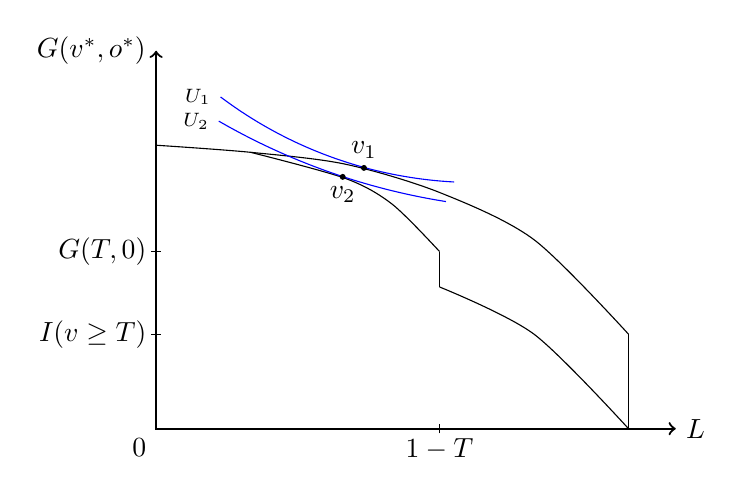
\begin{tikzpicture}[scale=0.6]
	% axis
	\draw[thick,<->] (0,8) node[left]{$G(v^*,o^*)$}--(0,0)--(11,0) node[right]{$L$};
	\node [below left] at (0,0) {$0$};
	% video incentive threshold
	\node [below] at (6,0) {$1-T$};
	\draw (6,-0.1) -- (6,0.1);

	% production frontier 1 - not incentivized
	\draw (10,0)--(10,2);
	\draw plot [smooth] coordinates {(10,2) (8,4) (6,5) (4,5.6) (2,5.85) (0,6)};

	% production frontier 2 - incentivized
	\draw plot [smooth] coordinates {(10,0) (8,2) (6,3)};
	\draw (6,3)--(6,3.75);
	\draw plot [smooth] coordinates {(6,3.75) (5,4.75) (4,5.3) (2,5.85)};

	% indifference curves
	% original
	\draw[blue] (4,5.65) arc[start angle=252, delta angle=15, radius=9cm];
	\draw[blue] (4,5.65) arc[start angle=252, delta angle=-19, radius=9cm] coordinate (u1);
	\node[left] at (u1) {\scriptsize $U_1$};
	% tangency
	\draw [fill] (4.4,5.52) circle [radius=.05];
	\node [above] at (4.4,5.52) {$v_1$};

	% new
	\draw[blue] (4,5.32) arc[start angle=252, delta angle=9, radius=14cm];
	\draw[blue] (4,5.32) arc[start angle=252, delta angle=-12, radius=14cm] coordinate (u2);
	\node[left] at (u2) {\scriptsize $U_2$};
	% tangency
	\draw [fill] (3.95,5.33) circle [radius=.05];
	\node [below] at (3.95, 5.33) {$v_2$};

	% grade incentive
	\node [left] at (0,3.75) {$G(T,0)$};
	\draw (-0.1,3.75) -- (0.1,3.75);
	\node [left] at (0,2) {$I(v \geq T)$};
	\draw (-0.1,2) -- (0.1,2);


	\end{tikzpicture}

	\caption{\textit{Above}: Demand curve for video watching as a function of leisure $L$. At $L=1-T$, the student maximizes grades $G(v,0)$ by spending all studying time watching videos, i.e. $v^*=T$. \textit{Below}: Student's utility maximization problem for the neoclassical model. The student maximizes her utility over leisure $L$ and grades $G$, which is a function of time allocated to video watching $v$ and her next best studying option $o$. The grade incentive $I$ is given to the student conditional on watching $T$ hours of videos (inner-time budget constraint) or, in the unincentivized case, given regardless of video watching (outer time-budget constraint).}
\end{center}
\end{figure}



\begin{figure}
\begin{center}
% Utility curves
\begin{tikzpicture}[scale=0.6]
% axis
\draw[thick,<->] (0,10) node[left]{$G(v^*,o^*)$}--(0,0)--(10,0) node[right]{$L$};
\node [below left] at (0,0) {$0$};
% production frontier 1
\draw (9,0)--(9,1);
\draw[domain=0:9, smooth] plot ({\x},{2*sqrt(9-\x) + 1});
% production frontier 2
\draw[domain=5:9, smooth] plot ({\x},{2*sqrt(9-\x) + 0});
\draw (5,4)--(5,4.7);
\draw[domain=0:5, smooth] plot ({\x},{2.2*sqrt(9-\x) + 0.3});
% indifference curves
% kink
\draw[blue] (5,4.7) arc[start angle=232, delta angle=10, radius=14cm];
\draw[blue] (5,4.7) arc[start angle=232, delta angle=-10, radius=14cm] coordinate (u1);
\node[above] at (u1) {$U_1$};
% tangency
\draw[blue] (6.5,4.2) arc[start angle=235, delta angle=15, radius=9cm];
\draw[blue] (6.5,4.2) arc[start angle=235, delta angle=-19, radius=9cm] coordinate (u2);
\node[above] at (u2) {$U_2$};
\end{tikzpicture}
% Isograde curves
\begin{tikzpicture}[scale=0.6]
	% axis
	\draw[thick,<->] (0,10) node[above]{$G(v^*,o^*)$}--(0,0)--(10,0) node[right]{$L$};
	\node [below left] at (0,0) {$0$};
	% Isograde curves
	\draw (4.45,5.3) to [out=-90, in=140] (5.75,3.2) to [out=-40, in=160] (7.7,2.2);

	\draw (4.15,4.3) to [out=-90, in=120] (4.55,3) to [out=-60, in=160] (7.4,1.1);

	\draw (0,6.45) to [out=0, in=115] (4.4,3.2) to [out=-65, in=90] (5.05,0);
\end{tikzpicture}

\caption{Student's utility maximization problem for the neoclassical model. The student maximizes her utility over leisure $L$ and grades $G$, which is a function of time allocated to video watching $v$ and her next best studying option $o$.}
\end{center}
\end{figure}

In the neoclassical model, the marginal return to grades of the incentived input is less than that of the outside option for the `compliers', or those induced by the incentive to consume at least a fixed level of the incentived input. This model predicts bunching at the incentivized level cutoff since compliers would prefer to spend their marginal hours on leisure or studying with their other method. This model predicts a strict increase in video watching and weak decrease in other studying and leisure consumption. It is ambiguous whether cumulative study time increases or decreases as this depends on relative utility benefits of leisure and grades and the returns to studying by each method. However, if cumulative study time remains constant or decreases, then exam performance should strictly decrease since students are now suboptimally allocating study time versus their first-best allocation when considering only marginal returns to studying. On the other hand, if cumulative study time increases, students may earn greater exam grades but achieve lower utility compared to baseline. Importantly, this model predicts that in subsequent quarters students return to their pre-incentive levels of studying.

In the imperfect information model, students' \textit{ex ante} allocations to each studying method are not necessarily first-best. Compliers update their priors about the returns to watching videos as they work towards hitting the minimum required level. At this cutoff, they make a decision whether to continue watching videos depending on their updated perceptions of the marginal benefit. Hence, bunching at the cutoff is predicted only if the updated marginal benefit at the cutoff is lower than the marginal benefit of the next best studying option or the marginal utility of leisure.

 that the marginal benefit at the cutoff is greater (lower) than the marginal benefit of their next best option

the incentive to watch videos will increase exam performance as long as total study time does not fall. A sharp prediction is that video watching will continue at the incentivized level in the absence of the grade incentive as students have learned an effective study tool. We also expect the treatment effect to be greater for students with more information problems and one plausible group is transfer students who are taking their first class at UC San Diego, their first upper division class and, typically, their first class under the quarter system (vs the semester system used by most California community colleges).

Finally, in the behavioral model, the instructor's inducement helps students stick to study plans. As long as total study time does not fall, the inducment will increase exam performance. In the absence of the inducement, a sharp prediction is that video watching will revert to pre-inducment levels.

In the empirical section, we test for the effects of being induced to watch the IMVH on exam scores and several other study methods students could use to learn microeconomics (lecture attendance, visits to a class-specific tutoring lab, use of a class discussion board, downloads from the class web page). We examine the effects of treatment on grades in other classes taken in the same quarter. We compare bunching of video watching across treatment status.  For a subset of our sample we have survey responses on total study time in the quarter and leisure time. Since the experiment was conducted in the first of a required sequence, we test for differences in video watching across treated and control students in the next class. 
% *****************************************************************
% Background
% *****************************************************************

\section{Related Literature and Contributions} \label{background}

Students have many time-consuming activities to help them learn including attending class, watching recorded lectures, reading the textbook, doing homework, attending office hours, etc. There are several empirical challenges to estimating the causal effects of a learning activity. First, the decision to use a study method is likely to be influenced by unobservable student characteristics, such as motivation or ability, that are also likely to affect how well students do on exams. To estimate the causal effects of a study method, researchers must address selection into using the study method. Second, most instructors have experience working with motivated students who want to improve their study strategies after a negative exam shock which suggests "dynamic selection" into the use of a study method. Dynamic selection means that including student fixed effects in class performance regressions will not uncover the causal effect of a study method and \textcite{oettinger2002} and \textcite{ss2008} provide empirical evidence of such dynamic selection.\footnote{\textcite{oettinger2002} finds that students close to a grade threshold before the final exam perform better on the final and \textcite{ss2008} find significantly larger effects of studying on student's first year grades in IV regressions than in OLS regressions and show that this difference is not driven by measurement error in the study variable which suggests that study hours are negatively correlated with the OLS residual.  They find no evidence that students who study more have lower permanent observed ability, as measured by ACT scores, and provide suggestive evidence that students tend to increase effort in semesters when semester-specific elements of grades are low.}  Third, learning activities are substitutable and inducements to use one study strategy may affect student use of another. In these cases, even randomized experiments will not identify the causal effect of a study method but will rather identify the causal effects of a study policy and all of the changes in behavior caused by the policy. The causal effects of an educational policy, such as requiring homework, are useful for educators considering how to design their classes but are less useful for students wanting to know the relative effectiveness of study strategies. Fourth, some study methods may change the instructor's teaching style.  For example, in \textcite{msc2019} many instructors reported that lecture capture changed the way they lecture.  Again, experiments randomly assigning student to classes taught one way versus another will not identify the causal effect of a study method if other aspects of learning transmission are simultaneously changed. %zack --is it worth discussing that a new study method may change the value of other study methods?  Staying with lecture capture, the existence of a copy of lecture likely changes the value of attending lecture.
A fifth empirical issue is that study strategies all take time and so most empirical research jointly test the effectiveness of a particular learning method and devoting more time to the course. It is possible that the primary benefit to students is simply devoting more time to learning the course material, regardless of the study method.

Our study uses a randomized control trial as well as a RD approach which solves issues (1) and (2).  Since we use within-class randomization, we solve issue (4).  Our study does not solve issues (3) and (5), however, we have empirical evidence on a large number of alternative study methods and test if the inducement to use the video book affected these other study methods to shed light on issue (3) and we have survey data on study time for the course for a selected sample of students which we use to test whether total study time for the couse differs across treated and control students to shed light on issue (5).

Attending class: \textcite{cl2008} estimate the average effect of attending lecture for those who attend lecture (average treatment effect on the treated). The same instructor taught two required public finance classes of size 67 students and 47 students.  The instructor provided identical PowerPoints to both classes after lecture, but did not lecture on randomly chosen topics to a randomly chosen class.  The outcome is whether the student answers a multiple choice exam question correctly.  Physically attending lecture involves transportation costs and this costly aspect of lecture is not captured by the authors since the exam score comparison is across students who were all in class.  However, this study does identify the effect of attending a remote lecture versus having a written explanation.

\textcite{dgm2010} analyze a policy where lecture attendance was voluntary before the midterm, but after the midterm, students scoring below the median were required to attend class. The policy affected 352 students taking three classes, two intermediate micro and one econometrics class. The policy led to a 36 percentage point increase in post-midterm attendance at the threshold. Using a regression discontinuity design, they find that a 10 percentage point increase in overall attendance results in a 0.17 standard deviation increase in the final exam score. They find no effect of the attendance policy on grades in other classes taken the same quarter, attending TA sections, homework scores, and the use of university tutors.
% Zack--They also found positive but not statistically significant spillover effects on other classes. They hypothesize could be due to fixed costs of coming to campus.
\textcite{ans2012} study section (as opposed to lecture) attendance across intermediate microeconomics, intermediate macroeconomics and econometrics for 444 students. The authors find that absenteism depends on day of week and time of day and, since students are randomly assigned to sections, use these variables as instruments for absenteeism. They also include student fixed-effects. They find significant attendance effects only for students in the top quantiles: missing 10 percent of sections results in a 1 percentage point performance loss. The authors have no information about other uses of the student's time, including attending the main lecture.

Effect of Homework: \textcite{ts2012} randomly require two-thirds of student in a Principles of Economics classes to complete one of three homework assignments for a grade while the other third may complete the homework, but it does not contribute to their grade. The outcome measure is exam performance on questions related to the three homework assignments. The authors use the score on the remaining exam questions as a control variable. They find significant effects pf homework on the first midterm but not the final exam. \textcite{gr2013} use within-class randomization to estimate the effects of required homework for 423 microeconomics principles students. A coin flip determined whether a student was in the treated group, where course points are based on both homework and exams, or in the control group, where all course points are based on exams. Treatment led to a 58 percentage point increase in completing all homework assignments and a 84 percentage point increase in completing the majority of homework assignments. They find that treated students are less likely to drop the class and score higher on the first two but not the last two exams. The average across the four exams is increased 5-6 percent by treatment and the control group GPA would increase from 2.44 to 2.68 if they had been required to do homework. They find three times larger treatment effects for students who initially fail the first exam (10 to 15 percent vs 4 to 6 percent increase in average test scores). The authors do not examine whether other uses of student time are affected by the homework policy.

Effect of Study time: In a convincing empirical paper on the effects of study time, \textcite{ss2008} examine 210 Berea College students who were randomly assigned a roommate. Students whose roomates brought a video game to college, earn lower grades and spend less time studying. They authors instrument for study time using presence of a roommate with a video game and find that a one hour increase in study time per day (a .67 standard deviation increase in their sample) has the same effect of first semester GPA as a 5.21 increase in the ACT (an increase of 1.4 standard deviations in their sample).

Other researchers have investigated using technology to improve learning. \textcite{abbm2020} conduct an experiment in Botswana during the COVID-19 pandemic and find that text messages and phone calls deployed as low cost, scalable learning technologies improved test scores by 0.16 to 0.29 standard deviations.

Effect of Recorded Lectures: An educational resource closely related to the IMVH is when instructors record their lectures and make them available to students. Recorded lectures have course administration information which the IMVH does not have. Compared to an IMVH video, recorded lectures are typically much longer, less organized, and may include components that do not work well when recorded, such as group work or class discussion.  \textcite{savage2009} taught two intermediate micro classes: one 42-student class had "talk and chalk" lectures and the other 45-student class used technology that allowed lecture capture which was then made available to the students. The author finds no significant differences in observed student characteristics across the two sections but exam performance was significantly higher across the classes.

Effect of Setting Goals:  \textcite{cgpr2020} explore the effect of having students set goals on class performance. They find that setting task-based goals, completing a specific number of online practice exams, improves student performance on exams. Those randomly assigned to complete task-based goals completed 0.102 of a standard deviation more practice exams and increased total course points by .068 of a standard deviation. The authors caution that it is important that the tasks are based on a productive study method. The authors also explored performance-based goals, getting dspecific grades in the course or on exams, did not have an effect on course points.  In the intervention studied in this class, the instructor gave the student a task-based goal, as opposed to the student setting theiwas set by the instructor as opposed to the student and there was a direct grade penalty to not acheiveing the goal.

This study adds to this body of research by studying the effectiveness of an educational innovation: a video textbook. We randomly assign half the students scoring below the mdican on the first midterm to a grading scheme which placed 4 percent, or 40 points, of the student's grade on watching 40 videos and down-weighted the first midterm by 4 percent.  This experiment allows two empirical strategies to test for causal effects: within class randomization for students scoring below the median on the first exam and a regression discontinuity approach at the median first exam score. We examine a large set of student study behaviors (lecture attendance, homework downloads from course web page, contributions to a discussion board, use of a class-specific tutoring lab) to determine if any of these study methods are substitutes or complements with video watching. We test for spillovers to other classes taken in the same quarter. We test for heterogeneous treatment effects using techniques that are robust to p-hacking. Finally, our research setting allows us to examine video views in the absence of the grade incentive in the next, required intermediate microeconomics class.

The Intermediate Microeconomics Video Handbook (IMVH) is a collection of 220 shortish videos that cover the material for a year-long intermediate microeconomics class. Most topics were covered by two videos: one video introduces the concepts more intuitively with verbal explanations and graphs and the other video has the more formal, calculus-based definitions. The videos were created by six UC San Diego faculty members with professional videographer and production support. Many videos were created using an innovative presentation technology, the "learning glass," where the instructor uses neon markers to write on a large sheet of glass that has lights embeded along the glass edge to make the colors pop. The remaining videos are PowerPoint presentations that faculty edit as they talk and the instructor's image is superimposed next to the PowerPoint. Videos are closed captioned and were checked by graduate student for accuracy. Given the complexity of the material, a key objective of the faculty was to keep the web interface clean and simple so as not to distract from the content. A second objective was to help students find what they want quickly and so the IMVH has both a table of contents and an index, there are time stamps for each video on the IMVH web site to let students know what is in each video, and the video captions are searchable so, while watching the video, students can seach for a keyword and jump to the part of a video with that word. The last objective was to help students know where various topics "live" in interemediate microeconomics (in consumer theory?  in producer theory? in welfare theory?) and so we keep the table of conntents on the left panel displayed at all times except when the student is watching a video. While we do not know of another textbook completely comprised of videos, the IMVH is similar both to the Khan Academy web site, to lecture podcasts, and to textbook web sites that incorporate instructional videos.


\begin{table}
	\caption{Information Transmission Formats.}
	\centering
	\begin{tabular}{c|c|c|c|c}
		\hline
		& Lecture & Book & Lecture Capture & IMVH\\
		\hline
		Instructor's time used & x & & &\\
		Instructor-Learner Interaction & x & & &\\
		Learner-Learner Interaction & x & & & \\
		Readable & & x & ? & x \\
		Scalable & ? & x & x & x\\
		Searchable & & x & & x \\
		Skimmable & & x & & x\\
		Stoppable & ? & x & x & x\\
		Watchable & x & & x & x\\

		\hline

	\end{tabular}
	\label{infotransmission}
\end{table}

Table 1 presents a classification of some options to present course material to students.\footnote{This table is a modification of a classification Martin Osborne proposed to one of the authors in an e-mail correspondance.} The IMVH differs from a traditional textbook because intructors explain, graph and derive mathematical results in much the same way one would in a lecture. The primary benefit of lecture is that students can stop the innstructor, ask questions and get answers in real time. There is also an important social aspect of lectures as students can interact with each other before, during and after lecture. The IMVH differs from lectures because students control the IMVH lecture: they can rewatch, speed up or slow down the lecture. Compared to a large lecture hall, all students can clearly see and hear the IMVH lecture. Finally, the IMVH is closed-captioned which may be particularly useful when English is not the first language of the instructor and/or the student. Compared to lecture capture, the IMVH presents the material differently than lecture

% *****************************************************************
% Data
% *****************************************************************

\section{Experimental Design} \label{expdesign}
We conducted the field experiment in four intermediate microeconomics courses, two in fall 2018 and two in fall 2019. The university is a large, diverse and selective public research four-year university. At this institution, intermediate microeconomics is a three quarter sequence required for students majoring in Economics. The experiment was conducted in the first course of the sequence, Micro A. For students who take Micro B the quarter after Micro A, we have exam grades and video viewing from Micro B.

Students were told about the experiment in the first lecture and the syllabus. At any time during the quarter, students could opt out of having their data included in the analysis sample.\footnote{Students opt out via an online form owned by the Teaching + Learning Commons (T+LC) so that neither the instructor nor research team could observe which students decided to opt out.} Students below the age of 18 at the start of the course as well as students enrolled via Extension were removed from the analysis dataset.\footnote{Students under the age of 18 were excluded per IRB protocol. We exlude Extension students because of their small number, their unknown and potentially very different preparation for the course compared to UC San Diego students, and we are missing most do not have information are so different from we do not know if they met the course prerequisites nor and }

The course is 10 weeks long and the experiment began four weeks into the ten week term following the grading of the first midterm exam, and as such, only students who took the first midterm were included in the experiment. Following the first midterm, students were assigned to one of three treatment arms: \textit{Incentive}, \textit{Control}, or \textit{Above median}. Students who scored below the median on the first midterm were randomly assigned to \textit{Incentive} or \textit{Control} whereas \textit{Above median} includes all other students in the experiment. Random assignment was issued using pairwise random assignment stratified on midterm score and year cohort (details on treatment assignment can be found in the Appendix). Students in the \textit{Incentive} arm received a grading scheme that encouraged watching videos during the rest of the term whereas \textit{Control} and \textit{Above the median} received the standard grading scheme that does not directly reward watching videos. The two different grading schemes are outlined in Table \ref{gradescheme}. Specifically, the \textit{Incentive} grading scheme requires that at least 40 of 48 eligible videos in the IMVH be watched to earn 4 percentage points towards the students' final grades\footnote{Watched in standard speed, 40 videos would require students to spend between 5.5 and 7.1 hours, depending on the length of videos chosen (on average 9.7 minutes in length each). Watching all incentivized videos in standard speed would require just shy of eight hours.}.
Notably, the 4 percentage points comes at the expense of the first midterm score, which had already occurred at the time of treatment assignment. Hence, we isolate the video incentive as the sole difference between treatment arms, giving us more confidence that the exclusivity assumption of our encouragement design holds. % TODO - move this to after the model explanations?

\begin{table}
	\caption{Grade scheme by treatment arm. \textit{Control} represents same grade scheme as \textit{Above median}. Differences between the two grade schemes in red.}
	\centering
	\begin{tabular}{ c|c|c }
		Assessment & Incentive & Control \\
		\hline
		$>$40 videos & \red{4\%} & \red{0\%} \\
		Midterm 1 & \red{18\%} & \red{22\%} \\
		Midterm 2 & 22\% & 22\% \\
		Final Exam & 50\% & 50\% \\
		Math Quiz & 1\% & 1\% \\
		Best 5 of 6 Quizzes & 5\% & 5\% \\
		\hline
		Total & 100\% & 100\% \\
	\end{tabular}
	\label{gradescheme}
\end{table}



Many non-majors take the class typically to either satisfy general education requirements or to explore majoring in Economics. Thus there are many students at the margin of majoring in economics in the class and so an important outcome is the likelihood the student takes the second class in the sequence. The other unique feature of this class is the large fraction of transfer students, for whom the class is not only their first experience with upper division coursework, but typically the first time taking a class under the quarter system (community colleges in the state are on the semester system), and their first class at a 4-year research university. Thus, we expect transfer students to have greater information problems.

While the experiment was conducted in the first class of the sequence (100A), we also have data from the second class in the sequence (100B). Fortunately, one instructor taught all four of the 100A classes (one of the authors) and another instructor taught all four of the 100B classes. Both instructors created half of the videos lectures for their course.

Enrollments are high enough that the 100A and 100B instructors both taught two classes back-to-back each quarter but offered all exams at a common time out-of-class. So we treat the two classes in a quarter the same but account for different years in the empirical analysis.

The 100A course had an identical structure across all quarters and years. In addition to a live lecture on T-Th (which were offered at two different times each day, either 11-12:30 or 12:30-2:00), students had access to weekly one-hour discussion sections run by Econ PhD students (including one of the authors), a tutoring lab staffed by both the graduate TAs and top undergraduates, weekly supplemental instruction sessions offered by undergraduates majoring in Economics and trained by the university in supplemental instruction, a discussion board (monitored by the instructor as well as the grad and undergrad TAs), four years of the instructor's old exams (no answers provided), weekly ungraded problem sets (with detailed answers), graded online quizzes on most Mondays, and a video handbook containing 220 short-ish videos covering the entire 100ABC sequence. This video handbook was created by the two instructors teaching 100A and 100B as well as four other faculty members who also regularly teach in the intermediate microeconomics sequence.

Students were told that final letter grades would not be affected by being in the experiment, so the two key experimental outcomes are the scores on the second midterm and on the final exam. Following [cite], we randomized the students into the experiment by sorting the students by the first midterm score, creating ordered student pairs and then choosing one of students in the pair randomly to be in the experiment.

Video ``watching" was based on opening the video, leaving it open for at least half the video length, and clicking a link at the end of the video which took students to a Qualtrics survey where they had to record their e-mail address on link at end of the video. Right after random assignment we surveyed students to make sure they knew which group they were in. Twice during the quarter we let students in the experiment know how many videos they had watched and how many more they needed to watch to earn the grade incentive.

In particular, we use an assessment (exam) to identify students most likely to be struggling with meeting the learning objectives of the course. We require a random sample of students who score below the median on the first midterm to partake in a required (for one's grade) study strategy consisting of watching at least 40 course-relevant supplementary videos. The videos were freely available to all students in the class and the instructor committed to having the course grade distribution identical across treatment and controls. To keep the weights on the second midterm and final exam, our primary outcome measures, the same across the treated and control groups, the first midterm was down-weighted for the treated group and the weight was put on watching 40 videos. Nearly all students in the treated group watched the 40 videos and treatment led to a X percentage point increase in video views relative to the control group. We find the grading policy led to an


% Estimating equations

We are primarily interested in the causal effect of watching videos on exam grades. The average causal effect of watching videos can be modeled using the potential outcome framework or Rubin Causal Model \parencite{ir2015}:

\begin{equation}
	\tau = E[Y_{it}(1) - Y_{it}(0)]
\end{equation}

where $\tau$ is the average causal effect of watching videos and $Y_{it}(1)$ and $Y_{it}(0)$ are the potential outcomes (e.g., exam scores) for a student $i$ in year $t$ who does and does not watch videos, respectively. We can observe treatment assignment for each student, $Z_{it} \in \{0,1\}$, as well as the observed outcome $Y_{it}(Z=z_{it})$ and a vector of pretreatment covariates $X_{it}$.

A student's decision to watch videos is endogenous, so we must rely on an exogenous instrument to calculate an unbiased estimate of $\tau$. By randomly assigning treatment that induces significantly greater video watching, the treatment indicator $Z_{it}$ satisfies the instrument validity and relevancy conditions required to estimate $\tau$ using an instrumental variable approach (citation). We calculate an estimate of $\tau$ using a two-stage least squares approach:

\begin{equation} \label{firststage_spec}
	v_{it} = \alpha Z_{it} + f(X_{it}) + e_{it}
\end{equation}
\begin{equation} \label{secondstage}
	y_{it} = \tau \hat{v}_{it} + g(X_{it}) + u_{it}
\end{equation}

where $\hat{v}_{it}$ is instrumented videos watched estimated by Equation \ref{firststage_spec}, $f()$ and $g()$ are generic functions through which $X_{it}$ affects $v_{it}$ and $y_{it}$, respectively, and $e_{it}$ and $u_{it}$ are model residuals assumed to be mean-zero conditional on observables. $\hat{\tau}$ is the estimate of the local average treatment effect (LATE) of watching videos local to those students induced by treatment to watch videos.

Under the assumptions of independence, monotonicity, and non-interference, $\hat{\tau}$ is an unbiased estimate of the LATE \parencite{ai1995}. Independence assumes that outcomes (e.g. grades) are only impacted by treatment through watching videos. This assumption could be violated if, for example, telling a student she is treated were to give her more confidence on subsequent exams during the quarter. Monotonicity, sometimes refered to as the ``no defiers assumption", is required because of two-sided noncompliance and requires that students assigned treatment are weakly more likely to watch videos than if they were assigned control. A violation of this assumption could occur if students get utility from rebelling against their assigned grade scheme. Non-interference, also known as the Stable Unit Treatment Value Assumption (SUTVA), assumes that each student's outcome depends only on their own treatment status and not the treatment status of their peers. Violations of SUTVA may include control students benefiting from having treated students in the same class (and perhaps studying together).

Although we believe excludability\footnote{While this assumption is not testable, we took care in the experimental design to make the treatment and control arms as similar as possible except for the grading schemes} and monotonicity\footnote{Though not testable directly, one testable implication of monotonicity is that the cumulative distribution function of videos watched for each treatment arm should not cross. Indeed, in Appendix Figure \ref{videocdf} shows that the two CDFs do not cross.} are reasonable assumptions, we have more pause about the non-interference assumption because of the potential for spillovers between students in the same class. If we had unlimited resources, a more robust experimental design would assign treatment at the class (or coarser) level, reducing the chance for interactions between treated and control students. However, given our resource constraints, assigning treatment at coarser levels would have resulted in insufficient statistical power to detect large effect sizes. Hence, we proceed acknowledging the potential for spillovers between students. We hypothesize that spillovers likely bias our estimates of the treatment effect \textit{downwards} as we believe control students are more likely to benefit from having well-studied peers than they are to lose from, for example, having peers too busy watching videos to join a study group.

We also estimate the average causal effects of being assigned to the \textit{Incentive} arm, or average Intention To Treat (ITT) effects. These are ITT estimates and not average treatment effect estimates because of non-compliance: some students in the treatment arm do not watch videos and some students in the control arm do watch videos. However, since the incentive itself in our setting is representative of how future instructors may require their students to use the IMVH, the ITT estimates are relevant for an instructor deciding whether to use a grade incentivize students to watch videos or simply make the videos available as a supplemental resource with no grade incentive.

Following the methods proposed by \textcite{robinson1988} and more recently \textcite{wa2018}, our primary estimating equation is the partially linear model:

\begin{equation}
	Y_{it} = \beta Z_{it} + f(X_{it}) + \epsilon_{it}
\end{equation}

where $Y_{it}$ is an outcome of interest (e.g. videos watched or test scores) for student $i$ in year $t$, $Z_{it} \in \{0,1\}$ is a treatment indicator, $f()$ is a generic function through which $X_{it}$, a vector of controls, affects $Y_{it}$, and $\epsilon_{it}$ is an unobserved residual. Following the Neyman-Rubin potential outcomes framework, $Y(Z=1|X) - Y(Z=0|X)$

To identify the causal effect parameter of interest, $\beta$, we make three assumptions: 1) \textit{treatment status unconfounded given controls}: $Z_{it} \perp \!\!\! \perp \Big(Y_{it}(Z=1), Y_{it}(Z=0)\Big) \Big| X_{it}$; 2)\textit{Excludability}: 3) \textit{Non-interference/Stable Unit Treatment Value Assumption (SUTVA)}:


% Neyman test of zero avg causal effect

\subsection{ITT}

We are interested in knowing the average effect of being assigned to the \textit{Incentive} arm on exam scores, which we will refer to as the Intent to Treat Effect (ITT). We will test the null hypothesis that being treated has zero effect against the alternative that being treated has a nonzero effect on exam scores. %positive effect?

We will estimate the ITT using Neyman's (\citeyear{neyman1923}) repeated sampling approach, considering each pair (block) a completely randomized experiment and averaging the results. We begin by estimating the point estimate of the ITT as the mean difference in outcomes across pairs:

\begin{equation} \label{itt_spec}
	\hat{\tau} = \frac{1}{J}\sum_{j=1}^{J} \hat{\tau_j} = \frac{1}{J}\sum_{j=1}^{J} y^\text{obs}_{j,I} - y^\text{obs}_{j,C}
\end{equation}

where $\hat{\tau}$ is the point estimate of the ITT, $J$ is the number of pairs in the sample, and $\hat{\tau_j} = y^{obs}_{j,I} - y^{obs}_{j,C}$ is the observed difference in outcome for pair $j$.

The point estimate $\hat{\tau}$ is appropriate if treatment is unconfounded by observable or unobservable variables. While this assumption is true in expectation given random assignment of treatment, as a robustness check we estimate specifications that control for differences in observed characteristics, described later in this paper.

Following Neyman's repeated sampling approach, the estimated standard error of $\hat{\tau}$ \citep{imai2008, ir2015, ai2017} is:

\begin{equation} \label{se_block}
	\hat{SE}(\hat{\tau}) = \Big(\frac{1}{J}\sum_{j=1}^{J} \hat{V}(\hat{\tau_j}) \Big)^\frac{1}{2}
\end{equation}

where $\hat{V}(\hat{\tau_j})$ is the estimated variance within block (pair) $j\in \{1,...,J\}$. This within-block variance given one control and one treated unit per block is (\cite{ir2015}, \cite{ai2017}):

\begin{equation} \label{v_block}
	\hat{V}(\hat{\tau_j}) = s_{j, I}^2 + s_{j, C}^2
\end{equation}

where $s_{j, I}$ and $s_{j, C}$ are the \textit{Incentive} and \textit{Control} sample variances within block $j$, respectively. Unfortunately, these sample variances are not estimable with only one unit in each arm per block. As such, we use the following estimator, which is conservative (confidence intervals wider) if there is heterogeneity in the treatment effect (\cite{imai2008}, \cite{ir2015}, \cite{ai2017}):

\begin{equation} \label{se_imai}
	\hat{SE}(\hat{\tau_j}) = \Big(\frac{1}{J(J-1)}\sum_{j=1}^{J} (\hat{\tau_j} - \hat{\tau})^2 \Big)^\frac{1}{2}
\end{equation}

\subsection{Treatment Effects at the Cutoff}

Because the probability of being assigned to the \textit{Incentive} arm changes discontinuously from 0.5 to 0 at the midterm score cutoff, our setting is appropriate for estimating local treatment effects using a regression discontinuity (RD) design \citep{tc1960, ap2008, il2008}. With this method, we compare students who scored just below the cutoff to those who scored just above the cutoff, two groups similar across pretreatment characteristics but different in treatment status, thereby providing an estimate of the treatment effect local to those who scored near the cutoff.

Since RD designs require that agents near the cutoff be similar across covariates except treatment status, a threat to validity is manipulation of the forcing variable (in our study, midterm score), which biases treatment effect estimates by nonrandom selection into treatment. This manipulation can occur if agents behave strategically to target a particular side of the cutoff, for example, scoring slightly higher than a published minimum SAT score for college admission. Since students in our experiment do not know the cutoff \textit{ex ante}, it is unlikely that students attempted to target a particular side of the midterm score cutoff\footnote{It would be surprising for students who value high grades to target the expected median score since any student capable of doing so would likely earn a higher grade in the course by scoring as high as possible on the midterm exam rather than strategically scoring just below the expected median cutoff.}. Ultimately, we must \textit{assume} continuity of the conditional means of the potential outcomes along the midterm score; however, we do not observe a discontinuity in any observable pretreatment covariate at the cutoff, which gives us further confidence that this assumption holds.

To estimate local treatment effects using a sharp RD, we return to the potential outcomes framework modeling the treatment effect $\tau(c)$ as the difference in expected outcomes at the cutoff $c$ along the forcing variable $x$:

\begin{equation} \label{rd_po}
	\tau(c) = \lim_{x \uparrow c} \mathbb{E}[Y_{it} | X_{it} = x] - \lim_{x \downarrow c} \mathbb{E}[Y_{it} | X_{it} = x] = \mathbb{E}[Y_{it}(1) | X_{it} = c] - \mathbb{E}[Y_{it}(0) | X_{it} = c]
\end{equation}

We estimate $\tau(c)$ using local low-order polynomials, per the advice of \textcite{gi2019}.

Sharp RD designs used in the literature frequently do not observe $Y(1)$ and $Y(0)$ for the same values of $x$. In our setting, however, we observe $Y(0)$ both above and below the cutoff. Hence, we need to assume continuity only for $Y(1)$ as we do not observe any outcomes for treated students scoring above the cutoff but \textit{do} observe outcomes for control students both above and below the cutoff.



% quantile regression?


% *****************************************************************
% Results
% *****************************************************************

\section{Results} \label{results}

In this section, we first establish that \textit{Incentive} and \textit{Control} arms are balanced on observable characteristics both when students were assigned treatment and when they took midterm and final exams. Second, we show that the grade-based encouragement worked, i.e. that students in the \textit{Incentive} arm watched significantly more videos than did their \textit{Control} peers. Third, we present results from the LATE and ITT specifications as described in the previous section. Finally, we estimate spillover effects in other courses during the experiment term as well as we the term following.

\subsection{Balance betweeen treatment arms}

\subsection{Relevancy of the encouragement instrument}

As described in the previous section, we use a Two-Stage Least Squares approach to estimate the LATE of watching videos on exam performance. We must check that our instrument is both valid and relevant to ensure this method will produce an unbiased estimate of the LATE \parencite{ir2015}. The validity condition is met by assigning the treatment arm at random conditional on observable characteristics, namely exam score and year of instruction. Additionally, Table \ref{balance_table_final} gives us further confidence that treatment status is uncorrelated with demographics. Next we check relevancy, i.e. whether treatment status generates significantly more video watching. Below in Table \ref{firststage_table} we present estimates from Equation \ref{firststage_spec} and find that being assigned to the \textit{Incentive} arm induces students to watch XX more videos than does being assigned to the \textit{Control} arm. The F-statistic is XX, far greater than 10, the generally accepted minimum value required to consider an instrument relevant.

\subsection{Estimation of causal effects}

First, we estimate the causal effect of being assigned to the \textit{Incentive} arm on exam scores (ITT). This estimate is relevant for educators interested in predicting how requiring videos will change exam scores in their classes using the same grade-based incentive implemented in our experiment. Second, we estimate the causal effect of watching videos on exam scores, which is of interest to educators deciding which teaching technologies to provide for their classes as well as to students choosing among different studying tools.

For both the ITTs and LATEs, we examine effects on the second midterm and final exams using both parametric methods (i.e. Equations \ref{itt_spec} and \ref{late_spec}) and nonparametric methods a la the repeated sampling framework of \textcite{neyman1923}% and Generalized Random Forests proposed by \textcite{wa2018}
. We check that our parametric results are robust to model specification by estimating Equations \ref{itt_spec} and \ref{late_spec} with and without $f(X_{it})$ as a vector of linear control variables chosen via the Post-Double-Selection procedure of \textcite{bch2014a}. To rule out differential attrition across treatment arms as a confounder, we fit the aforementioned models dropping any student whose matched pair attrited before the conclusion of the experiment.

\subsubsection{Effect of grade incentive on video watching}

Table \ref{firststage}

\subsubsection{Effect of treatment on exam scores}

Table \ref{secondstage}

\subsubsection{Substituion from other forms of studying}

Table \ref{spillover_studying}

\subsection{Spillover effects}

Here we estimate spillover effects to other other courses taken concurrently during the term of the experiment. We also estimate spillover effects to Micro B, the subsequent course in the intermediate microeconomics sequence. It is important to examine spillover effects

\subsubsection{Concurrent courses}

Table \ref{spillover_grades}

\subsubsection{Subsequent intermediate microeconomics course}

Table \ref{spillover_100b}



% *****************************************************************
% Discussion
% *****************************************************************

\section{Discussion} \label{discussion}


Students overwhelmingly report that they find the IMVH useful. But considering psychological learning theories, why might watching videos be effective?  The IMVH clearly facilitates interleaving (where students can easily review a variety of topics and not simply focus on the current topic which is the focus of lectures, problems sets, and quizzes), spaced practice (attend lecture and watch videos at some other time), learning information from different formats (IMVH presents information both verbally, graphically and algebraically) and using worked examples (IMVH includes many worked examples).  Again, it is also possible that the inducement to watch the IMVH simply led students to spend more times on the class.  Since we have no evidence that treated students reduced other study methods and watching the IMVH videos takes time, our empirical approach jointly tests the hypothesis that watching videos improves exam performance and that spending more time studying improves exam performance. However, the fact that treated students continued to watch more videos than the control students in Micro B suggests the videos were a uniquely useful study method.  Why do students at the median of midterm 1 score appear not to benefit from being induced to watch the videos?   This may be the result of a limitation of the running variable (midterm 1): there are few students near the midterm 1 median score which limits the power of an RD estimation strategy.  It may also be that students at the median know effective study strategies and being pushed to watch more videos is not helpful and so welfare reducing.  

\textcite{aws2015} review the literature on using technology to provide supplemental aids for students in traditional classrooms and conclude that there is little causal evidence that student acheivement is improved.  This study stands in contrast to this prior literature.

textcite{aws2015} review the literature on online instruction conclude that online instruction appears to have a negative effect on course grades and persistence.  A more recent paper byand a more recent paper usng an IV approach by \textcite{bflt2017} confirms , particularly for low-performaing students.  The IMVH is clearly the backbone for an online class as it includes all the videos one would require students to watch as part of an online course.  Would encouraging at-risk students to watch instructional videos in an online class be as effective as we find for a in-person class?  We consider this an important area for future research.   


\subsection{Limitations}

The present study has several limitations that should be considered before, for example, creating one's own video handbook and requiring students to use it. First, the population studied is students who score below the median on the first midterm of an intermediate microeconomics course at a large, highly-selective public research univerisity. The extent to which treatment effects vary by course, instructor, university, or along the midterm score distribution is beyond the scope of this paper. Additionally, the causal effects of watching videos that we estimate are local to compliers, i.e. students induced by the grade incentive to watch additional videos. We cannot recover the \textit{population} average treatment effect, though annecdotal evidence and economic theory both suggest that the population average treatment effect is likely greater than the LATE.%because control students watched many videos too even without incentive

Some researchers may wonder why we included only the bottom half of midterm scorers in the experiment instead of the entire class. Though we cannot estimate heterogeneity in treatment effects along the entire midterm distribution with our design, we believe this loss is justified by reduced risk of welfare losses by high performing students. The first midterm provides a signal of which students likely know for themselves how much and what kind of studying they should be doing. Coercing these high-type students to spend time with an alternative studying method is unlikely to be helpful and runs a higher risk of harming utility. On the other hand, students who have made manifest a need for alternative or more time studying stand to benefit the most from instructor-provided guidance.

Another consideration is the time frame during which the experiment took place, 2018 to 2019. About three months after the conclusion of our experiment, most students in the United States and all students at the studied university began remote learning as the coronavirus pandemic prompted stay-at-home orders. With increased experience learning via electronic media, it is possible that treatment effects will be higher in the future than we estimate in our paper. On the other hand, if students find online learning materials increasingly \textit{less} engaging, we may find the opposite.

Generalizability of our results. The experiment was conducted in intermediate microeconomics, a required course in all economics programs which typically has high failure rates.\footnote{At UC San Diego it is and at LSE it ranges from 12 percent in their least mathematical version to 24 percent in the more mathematical class, see https://www.lse.ac.uk/study-at-lse/The-General-Course/pdf/Choosing-economics-Course-guide-2020-21-HR-1.pdf} It is the first upper division class for many students and, for transfer students, also their first class in the university and under a XX percent quarter system. As such there may be large information problems about how to successfully study for the class under study and that there would be smaller effects of such an intervention in later classes.

Future research: most importantly, to see of our results hold up in other educational settings (e.g., different students, types of classes, instructors, and universities). We would like to examine the role of weekly deadlines instead of one final deadline at the end of the term, which may reduce the deleterious effects of binge-watching (though many top students also "binge watch" before midterm 2 and the final exam as they find this the most useful for reviewing the material.)


% *****************************************************************
% Conclusion
% *****************************************************************

\section{Conclusion} \label{conclusion}

We examine the effectiveness of an educational innovation, a video handbook composed of 220 brief instructional videos on intermediate microeconomic theory. We used random assignment of a grade-based incentive to experimentally vary takeup of the video handbook, and we found that greater takeup caused student to score significantly higher on exams. Specifically, we estimate that for students on the margin of watching videos, an additional hour of video watching causes students to score XX to XX standard deviations higher on exams.

Instructors may have concerns about making a resource such as the IMVH available if they believe students may substitute away from lectures or other more productive studying methods \textcite{kay2012}. Another concern is that forcing students to spend more time studying in one's class may cause worse performance in other classes. Our analysis provides some confidence that neither of these fears are first-order concerns. We do not find evidence that students decrease their consumption of other forms of studying, nor do we find that students perform worse in other courses during the same quarter. Our point estimates, though not statistically significantly different from zero, are positive for most alternative studying methods, suggesting that a potential mechanism of the videos may be helping students realize what they \textit{don't} know, whereas students who selectively study spend too much time on material they already know.

A final concern is one of welfare. In a neoclassical model, instructors cannot make their students better off by forcing on them quantities of studying they would not otherwise have chosen for themselves. In a behavioral model, which we think is more appropriate in our university classroom setting, instructors \textit{can} improve student welfare through intervention when information barriers and myopia lead to suboptimal time allocation decisions. We observe two phenomena that supports the latter model. First, treated students tend not to bunch at the cutoff for the grade incentive. Second, video consumption remains much higher among treated students in the term following conclusion of the experiment.

While there are many educational interventions that instructors could offer their students, the research on causal effects of educational interventions remains limited. Our study serves as an example of a feasible research design that runs a lower risk of generating welfare losses for high performing students than does a class-wide experiment. It is our hope, as educators ourselves, that more research be conducted on the effectiveness of pedagogical technologies.

\printbibliography

%%% TABLES

\clearpage
\begin{spacing}{1.0} 
\begin{table} \centering \caption{Baseline balance test, Final Exam sample} 
\label{balance_table_final} 
\resizebox{\linewidth}{!}{% 
\begin{threeparttable} 
\begin{tabular}{m{0.25\linewidth} *{7}{>{\centering\arraybackslash}m{0.095\linewidth}}}
\toprule 
 & \multicolumn{3}{c}{All students} & P-values & \multicolumn{2}{c}{Matched pairs}  & P-values  \\ 
\cmidrule(lr){2-4}\cmidrule(lr){6-7} 

             Variable & Above Median &  Control & Incentive & (3) - (2) &  Control & Incentive & (5) - (4) \\
\midrule
      \customlinespace Midterm 1 score &        2.049 &    0.153 &     0.057 &     0.291 &    0.177 &     0.170 &     0.938 \\
                      &      (0.025) &  (0.061) &   (0.069) &           &  (0.064) &   (0.065) &           \\
          \customlinespace Year = 2019 &        0.489 &    0.516 &     0.500 &     0.753 &    0.518 &     0.518 &     1.000 \\
                      &      (0.025) &  (0.037) &   (0.036) &           &  (0.039) &   (0.039) &           \\
       \customlinespace Cumulative GPA &        3.445 &    2.946 &     2.959 &     0.864 &    2.929 &     3.001 &     0.346 \\
                      &      (0.029) &  (0.044) &   (0.060) &           &  (0.047) &   (0.059) &           \\
          \customlinespace No cum. GPA &        0.231 &    0.359 &     0.332 &     0.583 &    0.367 &     0.313 &     0.299 \\
                      &      (0.021) &  (0.035) &   (0.034) &           &  (0.038) &   (0.036) &           \\
      \customlinespace Math quiz score &        0.599 &    0.071 &     0.152 &     0.396 &    0.061 &     0.157 &     0.338 \\
                      &      (0.043) &  (0.068) &   (0.066) &           &  (0.071) &   (0.071) &           \\
      \customlinespace Tutoring visits &        0.270 &    0.272 &     0.237 &     0.684 &    0.283 &     0.253 &     0.746 \\
                      &      (0.043) &  (0.061) &   (0.060) &           &  (0.066) &   (0.066) &           \\
       \customlinespace Videos watched &       13.292 &   13.418 &    13.658 &     0.856 &   13.729 &    13.789 &     0.966 \\
                      &      (0.682) &  (0.909) &   (0.953) &           &  (0.978) &   (1.023) &           \\
       \customlinespace Videos, unique &        9.793 &    9.783 &    10.111 &     0.704 &    9.795 &    10.181 &     0.674 \\
                      &      (0.432) &  (0.598) &   (0.622) &           &  (0.630) &   (0.665) &           \\
         \customlinespace Hours videos &        1.698 &    1.788 &     1.805 &     0.929 &    1.812 &     1.803 &     0.967 \\
                      &      (0.094) &  (0.130) &   (0.138) &           &  (0.138) &   (0.148) &           \\
 \customlinespace Hours videos, unique &        1.297 &    1.369 &     1.372 &     0.985 &    1.363 &     1.366 &     0.985 \\
                      &      (0.062) &  (0.093) &   (0.094) &           &  (0.098) &   (0.100) &           \\
                \customlinespace Asian &        0.701 &    0.696 &     0.653 &     0.376 &    0.711 &     0.633 &     0.129 \\
                      &      (0.022) &  (0.034) &   (0.035) &           &  (0.035) &   (0.038) &           \\
               \customlinespace Latinx &        0.060 &    0.141 &     0.158 &     0.654 &    0.139 &     0.169 &     0.448 \\
                      &      (0.012) &  (0.026) &   (0.027) &           &  (0.027) &   (0.029) &           \\
                \customlinespace White &        0.149 &    0.109 &     0.132 &     0.497 &    0.102 &     0.145 &     0.244 \\
                      &      (0.018) &  (0.023) &   (0.025) &           &  (0.024) &   (0.027) &           \\
      \customlinespace Other ethnicity &        0.089 &    0.054 &     0.058 &     0.882 &    0.048 &     0.054 &     0.804 \\
                      &      (0.014) &  (0.017) &   (0.017) &           &  (0.017) &   (0.018) &           \\
               \customlinespace Female &        0.393 &    0.348 &     0.405 &     0.253 &    0.337 &     0.404 &     0.212 \\
                      &      (0.024) &  (0.035) &   (0.036) &           &  (0.037) &   (0.038) &           \\
                 \customlinespace Male &        0.593 &    0.647 &     0.584 &     0.215 &    0.657 &     0.584 &     0.176 \\
                      &      (0.024) &  (0.035) &   (0.036) &           &  (0.037) &   (0.038) &           \\
             \customlinespace Transfer &        0.272 &    0.462 &     0.447 &     0.778 &    0.470 &     0.416 &     0.321 \\
                      &      (0.022) &  (0.037) &   (0.036) &           &  (0.039) &   (0.038) &           \\
         
\midrule 
Observations &          415 &      184 &       190 &           &      166 &       166 &           \\
\bottomrule
\end{tabular}
\Fignote{This table includes all students who completed the final exam. Descriptions of each variable can be found in Table \ref{controlvars_desc}. \textit{Male} and \textit{Female} are coded zero for nine students who do not report a gender. \textit{P-values} are reported for the Welch's t-test of equal means between the \textit{Control} and \textit{Incentive} arms. \Regnote} 
\end{threeparttable}}
\end{table} 
\end{spacing}

\clearpage
\begin{spacing}{1.0} 
\begin{table} \centering \caption{Effects of Grade Incentive on Video Watching} 
\label{firststage_table} 
\begin{threeparttable} 
\begin{tabular}{m{0.35\linewidth} *{5}{>{\centering\arraybackslash}m{0.1\linewidth}}}
\toprule
                               & Control Mean &       (1) &       (2) &       (3) &       (4) \\
\midrule
                        
\multicolumn{6}{l}{\textbf{Panel A}: By Midterm 2} \\ 

\customlinespace \indentrow{Videos} &        33.91 &  10.19\sym{***} &  10.54\sym{***} &   9.08\sym{***} &   9.58\sym{***} \\
                               &              &    (2.85) &    (3.12) &    (2.03) &    (2.19) \\
                 
\customlinespace \indentrow{Unique videos} &        23.13 &   6.63\sym{***} &   6.79\sym{***} &   5.97\sym{***} &   6.11\sym{***} \\
                               &              &    (1.54) &    (1.70) &    (0.98) &    (1.11) \\
               
\customlinespace \indentrow{Hours of videos} &         5.88 &   1.68\sym{***} &   1.72\sym{***} &   1.48\sym{***} &   1.55\sym{***} \\
                               &              &    (0.50) &    (0.55) &    (0.35) &    (0.38) \\
        
\customlinespace \indentrow{Hours of unique videos} &         3.85 &   1.10\sym{***} &   1.13\sym{***} &   0.99\sym{***} &   1.02\sym{***} \\
                               &              &    (0.25) &    (0.28) &    (0.16) &    (0.18) \\
                  
\midrule 
Observations &              &       395 &       362 &       395 &       362 \\
                        
\midrule 
\multicolumn{6}{l}{\textbf{Panel B}: By Final Exam} \\ 

\customlinespace \indentrow{Videos} &        53.09 &  39.25\sym{***} &  39.07\sym{***} &  38.57\sym{***} &  37.99\sym{***} \\
                               &              &    (4.06) &    (4.37) &    (3.40) &    (3.69) \\
                 
\customlinespace \indentrow{Unique videos} &        33.95 &  21.55\sym{***} &  21.08\sym{***} &  21.28\sym{***} &  20.49\sym{***} \\
                               &              &    (1.55) &    (1.66) &    (1.22) &    (1.27) \\
               
\customlinespace \indentrow{Hours of videos} &         8.93 &   6.30\sym{***} &   6.26\sym{***} &   6.18\sym{***} &   6.05\sym{***} \\
                               &              &    (0.69) &    (0.75) &    (0.57) &    (0.62) \\
        
\customlinespace \indentrow{Hours of unique videos} &         5.54 &   3.43\sym{***} &   3.36\sym{***} &   3.38\sym{***} &   3.26\sym{***} \\
                               &              &    (0.25) &    (0.27) &    (0.20) &    (0.21) \\
                  
\midrule 
Observations &              &       374 &       332 &       374 &       332 \\
 Treatment assignment controls &              &       Yes &        No &       Yes &       Yes \\
          Demographic controls &              &        No &        No &       Yes &       Yes \\
            Pair Fixed Effects &              &        No &        No &        No &       Yes \\
\bottomrule
\end{tabular}
\Fignote{Model (1) contains linear controls for midterm 1 score and year; (2) is the difference in means and standard errors calculated using the repeated sampling framework of Neyman (1923); (3) and (4) use the post-double-selection (PDS) procedure of \textcite{bch2014a} to select control variables then estimate treatment effects and standard errors. The control variables selected using PDS are listed in Table \ref{controlvars_selected_itt}. Models (2) and (4) include only students whose matched-pair did not attrite from the experiment. \textit{Control Mean} is the mean for the Control students included in models (1) and (3), which is nearly identical to the mean for the Control students included in models (2) and (4). \Regnote} 
\end{threeparttable}
\end{table} 
\end{spacing}

\clearpage
\begin{spacing}{1.0} 
 \def\sym#1{\ifmmode^{#1}\else\(^{#1}\)\fi} 
\begin{table} \centering \label{secondstage_table} 
 \caption{Effect of Videos on Grades} 
\begin{threeparttable} 
\begin{tabular}{m{0.35\linewidth} *{4}{>{\centering\arraybackslash}m{0.1\linewidth}}}
\toprule
                                     &      (1) &      (2) &      (3) &      (4) \\
\midrule
          \multicolumn{5}{l}{\textbf{Panel A}: Midterm 2 Score} \\ 
\indentrow{RF: Incentive}  &    0.18\sym{*} &    0.18\sym{*} &    0.18\sym{*} &    0.17\sym{*} \\
                                     &  (0.090) &  (0.094) &  (0.090) &  (0.096) \\
        \customlinespace \indentrow{2SLS: 10 Videos}  &   0.027\sym{*} &   0.027\sym{*} &   0.030\sym{*} &   0.029\sym{*} \\
                                     &  (0.015) &  (0.015) &  (0.015) &  (0.015) \\
 \customlinespace \indentrow{2SLS: 1 Hour of Videos}  &   0.224\sym{*} &   0.233\sym{*} &  0.238\sym{**} &   0.222\sym{*} \\
                                     &  (0.128) &  (0.138) &  (0.121) &  (0.124) \\
                        \customlinespace Observations &      395 &      362 &      395 &      362 \\
          \midrule 
 \multicolumn{5}{l}{\textbf{Panel B}: Final Exam Score} \\ 
\indentrow{RF: Incentive}  &   0.17\sym{**} &    0.17\sym{*} &   0.17\sym{**} &     0.14 \\
                                     &  (0.089) &  (0.103) &  (0.088) &  (0.103) \\
        \customlinespace \indentrow{2SLS: 10 Videos}  &  0.008\sym{**} &   0.008\sym{*} &  0.008\sym{**} &   0.009\sym{*} \\
                                     &  (0.004) &  (0.005) &  (0.004) &  (0.005) \\
 \customlinespace \indentrow{2SLS: 1 Hour of Videos}  &  0.074\sym{**} &   0.074\sym{*} &  0.074\sym{**} &    0.058 \\
                                     &  (0.038) &  (0.045) &  (0.037) &  (0.044) \\
                        \customlinespace Observations &      374 &      332 &      374 &      332 \\
       \midrule 
 Treatment assignment controls &      Yes &       No &      Yes &      Yes \\
                Demographic controls &       No &       No &      Yes &      Yes \\
                  Pair Fixed Effects &       No &       No &       No &      Yes \\
\bottomrule
\end{tabular}
\Fignote{This table reports coefficients on $Incentive_i$ from Equation \ref{late_spec} and $Video_i$ from Equation TBD. Test scores are measured in standard deviation units. Model (1) contains linear controls midterm 1 score and year; (2) is the difference in means and standard errors calculated using the repeated sampling framework of Neyman (1923); (3) and (4) use the post-double-selection (PDS) procedure of \textcite{bch2014a} to select control variables then estimate treatment effects and standard errors. The control variables selected using PDS are listed in Table \ref{controlvars_selected_itt}. Models (2) and (4) contain only students whose matched-pair did not attrite from the experiment.  \Regnote} 
 \end{threeparttable} 
 \end{table} 
 \end{spacing}

\clearpage
\begin{spacing}{1.0} 
\begin{table} \centering \caption{Spillover Effects of Incentive on Other Course Grades} 
\label{spillover_grades} 
\resizebox{0.9\linewidth}{!}{% 
\begin{threeparttable} 
\begin{tabular}{m{0.35\linewidth} *{5}{>{\centering\arraybackslash}m{0.1\linewidth}}}
\toprule
                               & Control Mean &     (1) &     (2) &     (3) &     (4) \\
\midrule
                   
\multicolumn{6}{l}{\textbf{Panel A}: Effects on Term GPA} \\ 

\customlinespace \indentrow{All classes} &         2.59 &  0.13\sym{**} &   0.13\sym{*} &   0.11\sym{*} &    0.10 \\
                               &              &  (0.06) &  (0.07) &  (0.06) &  (0.06) \\
                   &              &     373 &     332 &     373 &     332 \\
             
\customlinespace \indentrow{Excluding Micro A} &         2.75 &    0.10 &    0.11 &    0.09 &    0.10 \\
                               &              &  (0.07) &  (0.08) &  (0.07) &  (0.08) \\
                   &              &     370 &     329 &     370 &     329 \\
        
\customlinespace \indentrow{Excluding econ classes} &         2.99 &    0.06 &    0.09 &    0.06 &    0.08 \\
                               &              &  (0.10) &  (0.09) &  (0.09) &  (0.12) \\
                   &              &     315 &     278 &     315 &     278 \\
      
\customlinespace \indentrow{Econ classes ex. Micro A} &         2.44 &    0.07 &    0.02 &    0.07 &   -0.03 \\
                               &              &  (0.09) &  (0.08) &  (0.09) &  (0.12) \\
                   &              &     258 &     228 &     258 &     228 \\
           
\midrule 
\multicolumn{6}{l}{\textbf{Panel B}: Effects on classes passed} \\ 

\customlinespace \indentrow{Num. classes passed} &         3.28 &    0.08 &    0.09 &    0.05 &    0.02 \\
                               &              &  (0.09) &  (0.10) &  (0.09) &  (0.09) \\
       
\customlinespace \indentrow{Num. classes not passed} &         0.31 &    0.01 &   -0.01 &    0.01 &   -0.01 \\
                               &              &  (0.06) &  (0.06) &  (0.06) &  (0.06) \\
        
\customlinespace \indentrow{Num. classes withdrawn} &         0.05 &    0.01 &    0.01 &    0.01 &    0.01 \\
                               &              &  (0.03) &  (0.02) &  (0.03) &  (0.02) \\
       
\midrule 
\multicolumn{6}{l}{\textbf{Panel C}: Effects on class grade type} \\ 

\customlinespace \indentrow{Letter grade in Micro A} &         0.95 &   -0.04 &  -0.05\sym{*} &   -0.03 &   -0.04 \\
                               &              &  (0.03) &  (0.03) &  (0.02) &  (0.03) \\
   
\customlinespace \indentrow{\% classes taken for letter} &         0.93 &   -0.01 &   -0.01 &   -0.01 &   -0.01 \\
                               &              &  (0.01) &  (0.02) &  (0.01) &  (0.02) \\
         
\customlinespace \indentrow{\% classes taken P/NP} &         0.07 &    0.01 &    0.01 &    0.01 &    0.01 \\
                               &              &  (0.01) &  (0.02) &  (0.01) &  (0.02) \\
                  
\midrule 
Observations &              &     374 &     332 &     374 &     332 \\
 Treatment assignment controls &              &     Yes &      No &     Yes &     Yes \\
          Demographic controls &              &      No &      No &     Yes &     Yes \\
            Pair Fixed Effects &              &      No &      No &      No &     Yes \\
\bottomrule
\end{tabular}
\Fignote{This table reports coefficients on $Incentive_i$ from Equations \ref{eq:itt_spec}. GPA is measured on a 4.0 scale and is only affected by courses taken for a letter grade. Courses taken for Pass/No Pass (P/NP) have no bearing on GPA, nor do withdrawn courses. Model (1) contains linear controls for midterm 1 score and year; (2) is the difference in means and standard errors calculated using the repeated sampling framework of Neyman (1923); (3) and (4) use the post-double-selection (PDS) procedure of \textcite{bch2014a} to select control variables then estimate treatment effects and standard errors. The control variables selected using PDS are listed in Table \ref{controlvars_selected_itt}. Models (2) and (4) include only students whose matched-pair did not attrite from the experiment. \textit{Control Mean} is the mean for the Control students included in models (1) and (3), which is nearly identical to the mean for the Control students included in models (2) and (4). \Regnote}
\end{threeparttable}}
\end{table} 
\end{spacing}

\clearpage
\begin{spacing}{1.0} 
\begin{table} \centering \caption{Spillover Effects of Incentive on Other Studying} 
\label{spillover_studying} 
\begin{threeparttable} 
\begin{tabular}{m{0.39\linewidth} *{5}{>{\centering\arraybackslash}m{0.09\linewidth}}}
\toprule
                                  & Control Mean &     (1) &     (2) &     (3) &     (4) \\
\midrule
                Attendance checks &         5.91 &   -0.08 &   -0.09 &   -0.16 &   -0.10 \\
                                  &              &  (0.18) &  (0.17) &  (0.17) &  (0.18) \\
           Discussion board views &        49.81 &   10.64 &    8.51 &   10.64 &    3.69 \\
                                  &              &  (7.64) &  (8.25) &  (7.60) &  (8.05) \\
     Discussion board days online &        10.40 &    1.43 &    1.89 &    1.43 &    1.67 \\
                                  &              &  (1.55) &  (1.59) &  (1.54) &  (1.65) \\
 Discussion board questions asked &         0.53 &    0.32 &    0.30 &    0.32 &    0.30 \\
                                  &              &  (0.25) &  (0.30) &  (0.25) &  (0.31) \\
         Discussion board answers &         0.47 &    0.08 &    0.01 &    0.08 &   -0.02 \\
                                  &              &  (0.26) &  (0.28) &  (0.26) &  (0.28) \\
                  Tutoring visits &         0.41 &    0.05 &   -0.01 &    0.07 &    0.00 \\
                                  &              &  (0.13) &  (0.14) &  (0.12) &  (0.12) \\
                     
\midrule 
Observations &              &     374 &     332 &     374 &     332 \\
    Treatment assignment controls &              &     Yes &      No &     Yes &     Yes \\
             Demographic controls &              &      No &      No &     Yes &     Yes \\
               Pair Fixed Effects &              &      No &      No &      No &     Yes \\
\bottomrule
\end{tabular}
\Fignote{This table reports coefficients on $Incentive_i$ from Equations \ref{itt_spec}. There were seven \textit{Attendance checks} during the quarter. \textit{Tutoring visits} includes those after the first midterm. Model (1) contains linear controls for midterm 1 score and year; (2) is the difference in means and standard errors calculated using the repeated sampling framework of Neyman (1923); (3) and (4) use the post-double-selection (PDS) procedure of \textcite{bch2014a} to select control variables then estimate treatment effects and standard errors. The control variables selected using PDS are listed in Table \ref{controlvars_selected_itt}. Models (2) and (4) include only students whose matched-pair did not attrite from the experiment. \textit{Control Mean} is the mean for the Control students included in models (1) and (3), which is nearly identical to the mean for the Control students included in models (2) and (4). \Regnote} 
\end{threeparttable}
\end{table} 
\end{spacing}

\clearpage
\begin{spacing}{1.0} 
\begin{table} \centering \caption{Spillover Effects during Subsequent Quarter} 
\label{spillover_100b} 
\resizebox{0.8\linewidth}{!}{% 
\begin{threeparttable} 
\begin{tabular}{m{0.35\linewidth} *{5}{>{\centering\arraybackslash}m{0.1\linewidth}}}
\toprule
                               & Control Mean &       (1) &     (2) &       (3) &     (4) \\
\midrule
                
\multicolumn{6}{l}{\textbf{Panel A}: Videos during subsequent quarter} \\ 

\customlinespace \indentrow{Num. of videos} &        25.46 &  14.00\sym{***} &  12.78\sym{*} &  11.70\sym{***} &   11.35 \\
                               &              &    (4.45) &  (6.74) &    (4.24) &  (7.08) \\
            
\customlinespace \indentrow{Num. unique videos} &        19.77 &   9.87\sym{***} &  8.85\sym{**} &   8.25\sym{***} &  8.07\sym{**} \\
                               &              &    (3.03) &  (4.04) &    (2.92) &  (4.12) \\
               
\customlinespace \indentrow{Hours of videos} &         3.82 &   2.14\sym{***} &   1.88\sym{*} &   1.79\sym{***} &    1.70 \\
                               &              &    (0.68) &  (1.03) &    (0.64) &  (1.08) \\
           
\customlinespace \indentrow{Hours unique videos} &         2.90 &   1.51\sym{***} &  1.33\sym{**} &   1.27\sym{***} &  1.22\sym{**} \\
                               &              &    (0.45) &  (0.60) &    (0.44) &  (0.61) \\
                  
\midrule 
Observations &              &       211 &     108 &       211 &     108 \\
               
\midrule 
\multicolumn{6}{l}{\textbf{Panel B}: Effects on classes passed} \\ 

\customlinespace \indentrow{Midterm 1 score} &              &     -0.04 &   -0.24 &     -0.04 &   -0.30 \\
                               &              &    (0.13) &  (0.18) &    (0.13) &  (0.19) \\
                   &              &       213 &     112 &       213 &     112 \\
               
\customlinespace \indentrow{Midterm 2 score} &              &      0.00 &   -0.04 &      0.00 &    0.03 \\
                               &              &    (0.13) &  (0.20) &    (0.13) &  (0.21) \\
                   &              &       214 &     112 &       214 &     112 \\
              
\customlinespace \indentrow{Final exam score} &              &      0.12 &    0.00 &      0.12 &    0.23 \\
                               &              &    (0.14) &  (0.18) &    (0.14) &  (0.23) \\
                   &              &       211 &     108 &       211 &     108 \\
                  
\midrule 
\multicolumn{6}{l}{\textbf{Panel C}: Effects on class grade type} \\ 

\customlinespace \indentrow{Took Micro B} &         0.61 &     -0.07 &   -0.07 &     -0.07 &   -0.08 \\
                               &              &    (0.05) &  (0.05) &    (0.05) &  (0.06) \\
           
\customlinespace \indentrow{Num. classes passed} &         3.46 &     -0.07 &   -0.05 &     -0.07 &   -0.04 \\
                               &              &    (0.11) &  (0.12) &    (0.11) &  (0.12) \\
       
\customlinespace \indentrow{Num. classes not passed} &         0.23 &      0.07 &    0.08 &      0.07 &    0.07 \\
                               &              &    (0.06) &  (0.06) &    (0.06) &  (0.06) \\
        
\customlinespace \indentrow{Num. classes withdrawn} &         0.06 &      0.04 &    0.04 &      0.04 &    0.03 \\
                               &              &    (0.03) &  (0.03) &    (0.03) &  (0.03) \\
                  
\midrule 
Observations &              &       374 &     332 &       374 &     332 \\
 Treatment assignment controls &              &       Yes &      No &       Yes &     Yes \\
          Demographic controls &              &        No &      No &       Yes &     Yes \\
            Pair Fixed Effects &              &        No &      No &        No &     Yes \\
\bottomrule
\end{tabular}
\Fignote{This table reports coefficients on $Incentive_i$ from Equations \ref{eq:itt_spec}. Panel A restricts the sample to those who completed both the first and second microeconomics courses (Micro A and B). Panel C includes those who completed the first microeconomics course (Micro A). Test scores are measured in standard deviation units. Model (1) contains linear controls for midterm 1 score and year; (2) is the difference in means and standard errors calculated using the repeated sampling framework of Neyman (1923); (3) and (4) use the post-double-selection (PDS) procedure of \textcite{bch2014a} to select control variables then estimate treatment effects and standard errors. The control variables selected using PDS are listed in Table \ref{controlvars_selected_itt}. Models (2) and (4) include only students whose matched-pair did not attrite from the experiment. \textit{Control Mean} is the mean for the Control students included in models (1) and (3), which is nearly identical to the mean for the Control students included in models (2) and (4). \Regnote}
\end{threeparttable}}
\end{table} 
\end{spacing}

%%% PLOTS

% Time series

% video CDF

% *****************************************************************
% Appendix
% *****************************************************************

\clearpage

\section*{Appendix}

\renewcommand{\thesubsection}{\Alph{subsection}}

\setcounter{table}{0}
\renewcommand{\thetable}{A\arabic{table}}

\subsection{Additional experiment details}

In this section we outline additional experiment details that could prove useful for replication or understanding our analysis choices.

\subsubsection{Randomization} \label{a_randomization}
Students were assigned to treatment arms using a matched pairs design, a special case of blocked randomization in which each block contains exactly two units, one treated and one control. Several authors detail how matched pair designs can improve the \textit{ex ante} precision of treatment effect estimates (versus complete randomization) by matching treatment units whose potential outcomes are similar (e.g. \cite{ir2015}, \cite{ai2017}). The

Additionally, we were unable to observe most pretreatment covariates until after the experiment had concluded because of student privacy considerations, thereby making it impossible to block on these variables. We learned from the previous cohorts' data that between the first midterm score and math quiz score, both observable at the time of randomization, the midterm score predicted significantly more variation in the final exam score. Hence, we stratified on midterm score when assigning treatment. While we could have used an alternative method (e.g. matching methods) that take into consideration multiple covariates when assiging treatment, we opted for a simpler design given the high correlation between midterm and math quiz score and the comparatively high number of missing observations for the latter assessment (the math quiz was given on the second class day and so before some students enrolled in the class).

We assigned treatment shortly after issuing midterm exam grades, which occured during the fourth week of the quarter. To assign treatment, we ordered the students by exam score, then paired students along this ordering for students below the median. Within pairs, we randomly assigned one student to \textit{Incentive}, the other to \textit{Control}. By construction, these two arms were \textit{ex ante} balanced on midterm exam score, and we verified at time of treatment that the arms were also balanced on math quiz score. Since this randomization was performed independently across year cohorts, by construction, the samples were also balanced on year.

Although our treatment assignment method provides a better chance of balance than does simple random sampling, by random chance and through non-random attrition, it is possible that the two treatment arms vary on \textit{ex post} observable and unobservable covariates that are correlated with the outcomes of interest, thereby confounding our treatment effect estimates. The primary cause of attrition was withdrawing from the course, which reduced our sample by XX students before the second midterm and XX students before the final exam. A XX\% rate of withdraw is in line with the withdraw rates observed in previous quarters. Another cause of attrition, albeit not from the course, is age: four students under the age of 18 during the experiment were removed from the analysis dataset. Additionally, seven students opted out of having their data included in the experiment analysis.

Since neither the students' intent to withdraw, age, nor opt-out preferences were observable at the time of treatment assignment, we could not \textit{ex ante} balance this attrition across treatment arms. If students attrited non-randomly, that is, decided to attrite depending on their treatment status, then our treatment effect estimates would be biased. Fortunately, despite XX\% of students attriting before the second midterm and XX\% before the final exam, the two treatment arms below the median are balanced on nearly all observable pretreatment covariates, as shown in Table \ref{balance_table_final}, which gives us confidence that the \textit{Control} arm is a good counterfactual for the \textit{Incentive} arm.

\subsubsection{Selection of control variables} \label{a_selection}

In this section we discuss how we select control variables included in linear models estimated in this paper.
% In our nonparametric estimation strategies that use generalized random forests, the algorithms implicitly select control variables that matter most for treatment heterogeneity and explaining variance in the outcome variables of interest (see Appendix \ref{a_grf}).

Equation \ref{itt_spec} includes a vector of control variables related linearly to the outcomes of interest. Although $d_i$, the treatment indicator is randomly assigned and in expectation $d_i$ is orthogonal to all observed and unobserved pretreatment covariates, in small samples stochastic imbalances can occur, which if controlled for can reduce bias of the treatment effect estimator \parencite{ai2017}. Even if perfect balance is achieved, controlling for orthogonal covariates can improve precision of the treatment effect estimator if the covariates can predict unexplained variance in the outcome.

By definition it is not possible to guarantee balance on unobserved covariates. As discussed in Appendix \ref{a_randomization}, we mechanically balanced the treatment arms on first midterm score, one of the few observables at the time of treatment assignment, with our knowledge from previous cohorts' data that the first midterm score explains a significant amount of variance in final exam score. Hence, in our estimation strategies including controls, we always include the first midterm score and year, following the recommendations of \textcite{bm2009} to control for all covariates used to seek balance when assigning treatment.

For variables unobservable at time of randomization but observable at time of analysis, we lack the luxury of guaranteed balance by construction, nor is it clear \textit{ex ante}, beyond our intuition, which will predict variation in the outcome variables of interest. On one hand, failing to control for valid predictors reduces statistical power. On the other hand, hand-picking control variables increases researcher degrees of freedom, risking increasing the prevalence of Type I errors \parencite{sns2011}. As such, in addition to a model without controls beyond the ones used for treatment assignment (year and midterm score), we fit a second model that includes a vector of linear controls chosen using the post-double-selection (PDS) procedure introduced by \textcite{bch2014a}.

PDS is a two step process in which first, model covariates are selected in an automated, principled fashion, and second, the model coefficients of interest are estimated while controlling for those selected covariates. The first step involves predicting, separately, both the outcome of interest (e.g., videos watched) and treatment status using lasso regression, which shrinks coefficient estimates towards zero. Note that since treatment is randomly assigned, the lasso should shrink most, if not all, of the coefficients towards zero when predicting treatment status. Next, the researcher takes the union of all covariates with non-zero coefficients and includes these covariates as controls in her model. With her control variables selected, she can now estimate treatment effects with reduced bias relative to including controls with less empirical rationale.

In Table \ref{controlvars_desc} below, we describe all covariates observable in our study. In Table \ref{controlvars_selected_itt}, we describe the covariates selected as controls for estimating the effect of treatment on each outcome variable of interest. All models include either pair fixed effects or year and midterm score as controls. To ensure these controls are ``selected" by the PDS procedure, we partialed out these controls from the first step prediction models by residualizing both sides of the equation as described in \textcite{bch2014b}.

\clearpage

\begin{spacing}{1.0} 
\begin{table} \centering \caption{Baseline balance test, Midterm 2 sample} 
\label{balance_table_mid2} 
\resizebox{\linewidth}{!}{% 
\begin{threeparttable} 
\begin{tabular}{m{0.25\linewidth} *{7}{>{\centering\arraybackslash}m{0.095\linewidth}}}
\toprule 
 & \multicolumn{3}{c}{All students} & P-values & \multicolumn{2}{c}{Matched pairs}  & P-values  \\ 
 \cmidrule(lr){2-4}\cmidrule(lr){6-7} 

             Variable & Above Median &  Control & Incentive & (3) - (2) &  Control & Incentive & (5) - (4) \\
\midrule
      \customlinespace Midterm 1 score &        2.048 &    0.116 &     0.037 &     0.398 &    0.139 &     0.131 &     0.933 \\
                      &      (0.025) &  (0.063) &   (0.068) &           &  (0.065) &   (0.066) &           \\
          \customlinespace Year = 2019 &        0.492 &    0.513 &     0.500 &     0.797 &    0.514 &     0.514 &     1.000 \\
                      &      (0.025) &  (0.036) &   (0.035) &           &  (0.037) &   (0.037) &           \\
       \customlinespace Cumulative GPA &        3.445 &    2.944 &     2.948 &     0.965 &    2.942 &     2.992 &     0.487 \\
                      &      (0.029) &  (0.043) &   (0.058) &           &  (0.045) &   (0.056) &           \\
          \customlinespace No cum. GPA &        0.230 &    0.368 &     0.332 &     0.452 &    0.365 &     0.320 &     0.377 \\
                      &      (0.021) &  (0.035) &   (0.033) &           &  (0.036) &   (0.035) &           \\
      \customlinespace Math quiz score &        0.592 &    0.037 &     0.106 &     0.471 &    0.054 &     0.137 &     0.396 \\
                      &      (0.044) &  (0.070) &   (0.065) &           &  (0.071) &   (0.068) &           \\
          \customlinespace PSET visits &        0.269 &    0.259 &     0.223 &     0.655 &    0.276 &     0.232 &     0.612 \\
                      &      (0.042) &  (0.059) &   (0.056) &           &  (0.062) &   (0.061) &           \\
       \customlinespace Videos watched &       13.228 &   13.368 &    13.777 &     0.750 &   13.663 &    13.729 &     0.961 \\
                      &      (0.681) &  (0.886) &   (0.931) &           &  (0.929) &   (0.986) &           \\
       \customlinespace Videos, unique &        9.746 &    9.689 &    10.188 &     0.554 &    9.845 &    10.116 &     0.760 \\
                      &      (0.431) &  (0.580) &   (0.611) &           &  (0.606) &   (0.644) &           \\
         \customlinespace Hours videos &        1.690 &    1.782 &     1.825 &     0.818 &    1.827 &     1.804 &     0.906 \\
                      &      (0.093) &  (0.127) &   (0.135) &           &  (0.133) &   (0.142) &           \\
 \customlinespace Hours videos, unique &        1.291 &    1.355 &     1.387 &     0.802 &    1.382 &     1.364 &     0.897 \\
                      &      (0.062) &  (0.090) &   (0.092) &           &  (0.095) &   (0.096) &           \\
                \customlinespace Asian &        0.700 &    0.694 &     0.668 &     0.581 &    0.713 &     0.652 &     0.215 \\
                      &      (0.022) &  (0.033) &   (0.033) &           &  (0.034) &   (0.036) &           \\
               \customlinespace Latinx &        0.060 &    0.135 &     0.158 &     0.506 &    0.133 &     0.166 &     0.377 \\
                      &      (0.012) &  (0.025) &   (0.026) &           &  (0.025) &   (0.028) &           \\
                \customlinespace White &        0.151 &    0.114 &     0.124 &     0.765 &    0.105 &     0.138 &     0.336 \\
                      &      (0.018) &  (0.023) &   (0.023) &           &  (0.023) &   (0.026) &           \\
      \customlinespace Other ethnicity &        0.089 &    0.057 &     0.050 &     0.741 &    0.050 &     0.044 &     0.804 \\
                      &      (0.014) &  (0.017) &   (0.015) &           &  (0.016) &   (0.015) &           \\
               \customlinespace Female &        0.393 &    0.342 &     0.391 &     0.312 &    0.343 &     0.392 &     0.328 \\
                      &      (0.024) &  (0.034) &   (0.034) &           &  (0.035) &   (0.036) &           \\
                 \customlinespace Male &        0.592 &    0.653 &     0.604 &     0.316 &    0.652 &     0.602 &     0.329 \\
                      &      (0.024) &  (0.034) &   (0.034) &           &  (0.036) &   (0.036) &           \\
             \customlinespace Transfer &        0.271 &    0.477 &     0.455 &     0.673 &    0.470 &     0.436 &     0.528 \\
                      &      (0.022) &  (0.036) &   (0.035) &           &  (0.037) &   (0.037) &           \\
         \midrule 
 Observations &          417 &      193 &       202 &           &      181 &       181 &           \\
\bottomrule
\end{tabular}
\Fignote{This table includes all students who completed the second midterm. Descriptions of each variable can be found in Table \ref{controlvars_desc}. \textit{Male} and \textit{Female} do not include nine students who do not report a gender. \textit{P-values} are reported for the Welch's t-test of equal means between the \textit{Control} and \textit{Incentive} arms. \Regnote} 
\end{threeparttable}}
\end{table} 
\end{spacing}

\clearpage

\begin{spacing}{1.0}\centering 
\begin{longtable}{p{0.3\linewidth} p{0.6\linewidth}}
\caption{Description of control variables eligible for selection a la Belloni et al (2014).}\label{controlvars_desc}\\
\toprule
        Variable &                                              Description \\
\midrule
\endhead
\midrule
\multicolumn{2}{r}{{Continued on next page}} \\
\midrule
\endfoot

\bottomrule
\endlastfoot
 Midterm 1 score &                               Score on the first midterm \\
     Year = 2019 &                   1 if course taken in 2019, 0 otherwise \\
  Cumulative GPA &        Cumulative GPA from prior term, 0 if not observed \\
     No cum. GPA &              1 if Cumulative GPA unobserved, 0 otherwise \\
 Math quiz score &       Score on a quiz assessing prerequisite math skills \\
     PSET visits &            Number of PSET visits as of the first midterm \\
  Videos watched &  Number of unique videos watched as of the first midterm \\
    Hours videos &   Hours of unique videos watched as of the first midterm \\
           Asian &                     1 if ethnicity is Asian, 0 otherwise \\
          Latinx &                    1 if ethnicity is Latinx, 0 otherwise \\
           White &                     1 if ethnicity is White, 0 otherwise \\
          Female &                                 1 if female, 0 otherwise \\
        Transfer &                       1 if transfer student, 0 otherwise \\
\end{longtable}
\end{spacing}

\clearpage

\begin{spacing}{1.0} 
\begin{ThreePartTable} 
\begin{TableNotes} 
\item \textit{Note}: Controls chosen via the PDS procedure of \textcite{bch2014a}. In the \textit{All Observations} model, \textit{Midterm 1 score} and \textit{Year = 2019} are additionally included as controls. In the \textit{Fixed Effects} model, pair fixed effects and \textit{Midterm 1 score} are included. All control variables are measured before the start of the experiment, e.g. \textit{Hours videos} is the hours of videos watched as of the first midterm.
\end{TableNotes} 
\footnotesize 
 \begin{longtable}{p{0.07\linewidth} >{\hangindent=1em}p{0.38\linewidth} p{0.22\linewidth} p{0.22\linewidth}}
\caption{ITT model controls selected via post-double-selection}\label{controlvars_selected_itt}\\
\toprule
      Table &                          Dependent Variable &                  Controls,\newline All Observations &                                                         Controls,\newline Fixed Effects \\
\midrule
\endfirsthead 
\multicolumn{4}{r}{{Table \ref{controlvars_selected_itt} (continued)}} \\
\toprule 
 \endhead
\midrule
\multicolumn{4}{r}{{Continued on next page}} \\
\midrule
\endfoot

\bottomrule
\insertTableNotes 
\endlastfoot
    Table 1 &                Hours unique videos by Final &                         Hours videos\newline Videos &                                                             Hours videos\newline Videos \\
            &               Hours unique videos by Mid. 2 &                                        Hours videos &                                                             Hours videos\newline Videos \\
            &                       Hours videos by Final &                                        Hours videos &                                                                            Hours videos \\
            &                      Hours videos by Mid. 2 &                                        Hours videos &                                         Hours videos\newline PSET visits\newline Videos \\
            &             Num. unique videos before Final &                         Hours videos\newline Videos &                                                                                  Videos \\
            &            Num. unique videos before Mid. 2 &                         Hours videos\newline Videos &                                                                                  Videos \\
            &                    Num. videos before Final &                         Hours videos\newline Videos &                                                             Hours videos\newline Videos \\
            &                   Num. videos before Mid. 2 &                         Hours videos\newline Videos &                                         Hours videos\newline PSET visits\newline Videos \\
    \midrule 
Table 2 &                            Final exam score &                                                None &                                                        Math quiz score\newline Transfer \\
            &                             Midterm 2 score &                                                None &                                                                         Math quiz score \\
    \midrule 
Table 3 &                                 All classes &                                      Cumulative GPA &                                 Cumulative GPA\newline Math quiz score\newline Transfer \\
            &                    Econ classes ex. Micro A &                                                None &                                                         Cumulative GPA\newline Transfer \\
            &                           Excluding Micro A &                                      Cumulative GPA &                                                                                Transfer \\
            &                      Excluding econ classes &                                                None &                                                                                    None \\
            &                     Letter grade in Micro A &      Cumulative GPA\newline Latinx\newline Transfer &                                                                          Cumulative GPA \\
            &                     Num. classes not passed &                                                None &                                                                                    None \\
            &                         Num. classes passed &                     Cumulative GPA\newline Transfer &                                                         Cumulative GPA\newline Transfer \\
            &                     Num. classes taken P/NP &                                              Latinx &                                                                                  Latinx \\
            &               Num. classes taken for letter &                  Cumulative GPA\newline No cum. GPA &                                                                          Cumulative GPA \\
            &                      Num. classes withdrawn &                                                None &                                                                                    None \\
            &                       Num. units taken P/NP &                                              Latinx &                                                                                  Latinx \\
            &           Num. units taken for letter grade &                  Cumulative GPA\newline No cum. GPA &                                                                          Cumulative GPA \\
            &                        Num. units withdrawn &                                                None &                                                                                    None \\
            &                       \% classes taken P/NP &                                                None &                                                                                  Latinx \\
            &                 \% classes taken for letter &                                                None &                                                                                  Latinx \\
    \midrule 
Table 4 &                           Attendance checks &  Female\newline Math quiz score\newline PSET visits &                                                                             PSET visits \\
            &                         Num. Piazza answers &                                                None &                                                                                    None \\
            &                     Num. Piazza days online &                                                None &                                                                                    None \\
            &                 Num. Piazza questions asked &                                                None &                                                                                    None \\
            &                           Num. Piazza views &                                                None &                                                                                   Asian \\
            &                         Num. of PSET visits &                                         PSET visits &                                                                             PSET visits \\
    \midrule 
Table 5 &                             Hours of videos &                                        Hours videos &  Hours videos\newline Latinx\newline Math quiz score\newline PSET visits\newline Videos \\
            &                             Midterm 1 score &                                                None &                                           Latinx\newline Math quiz score\newline Videos \\
            &                             Midterm 2 score &                                                None &                             Asian\newline Latinx\newline Math quiz score\newline Videos \\
            &                     Num. classes not passed &                                                None &                                                                                    None \\
            &                         Num. classes passed &                                                None &                                                                                    None \\
            &                     Num. classes taken P/NP &                                                None &                                                                                Transfer \\
            &               Num. classes taken for letter &                                                None &                                                                             No cum. GPA \\
            &                      Num. classes withdrawn &                                                None &                                                                                    None \\
            &                              Num. of videos &                                        Hours videos &  Hours videos\newline Latinx\newline Math quiz score\newline PSET visits\newline Videos \\
            &                       Num. units taken P/NP &                                                None &                                                                                Transfer \\
            &           Num. units taken for letter grade &                                                None &                                                                                    None \\
            &                        Num. units withdrawn &                                                None &                                                                                    None \\
            &                                    Term GPA &                                      Cumulative GPA &                                                      Cumulative GPA\newline PSET visits \\
            &  Term GPA, econ courses ex. Micro B, winter &                                                None &                                                                         Math quiz score \\
            &                       Term GPA, ex. Micro B &                                      Cumulative GPA &                                                      Cumulative GPA\newline PSET visits \\
            &                  Term GPA, ex. econ courses &                                                None &                                                                             PSET visits \\
            &                                Took Micro B &                                                None &                                                                         Math quiz score \\
            &                       \% classes taken P/NP &                                                None &                                                            No cum. GPA\newline Transfer \\
            &                 \% classes taken for letter &                                                None &                                                            No cum. GPA\newline Transfer \\
 Table None &                            Final exam score &                                                None &                                           Latinx\newline Math quiz score\newline Videos \\
            &                         Hours unique videos &                                        Hours videos &  Hours videos\newline Latinx\newline Math quiz score\newline PSET visits\newline Videos \\
            &                          Num. unique videos &                                        Hours videos &  Hours videos\newline Latinx\newline Math quiz score\newline PSET visits\newline Videos \\
            &                                Pass Micro B &                                                None &                                           Latinx\newline Math quiz score\newline Videos \\
\end{longtable}

\end{ThreePartTable} 
\end{spacing}

\clearpage

\begin{spacing}{1.0} 
\begin{table} \centering \caption{LATE model controls selected via post-double-selection} 
\label{controlvars_selected_iv} 
\resizebox{\linewidth}{!}{% 
\begin{threeparttable} 
\begin{tabular}{p{.25\linewidth} p{0.3\linewidth} p{0.22\linewidth} p{0.22\linewidth}}
\toprule
Dependent Variable &          Instrumented &                                           Controls,\newline All Observations & Controls,\newline Fixed Effects \\
\midrule
  Final exam score &  Hours videos, unique &         Hours videos\newline Math quiz score\newline Transfer\newline Videos &     Hours videos\newline Videos \\
  Final exam score &        Videos, unique &                                                  Hours videos\newline Videos &     Hours videos\newline Videos \\
   Midterm 2 score &  Hours videos, unique &  Hours videos\newline Math quiz score\newline Tutoring visits\newline Videos &                    Hours videos \\
   Midterm 2 score &        Videos, unique &                                                  Hours videos\newline Videos &     Hours videos\newline Videos \\
\bottomrule
\end{tabular}
\Fignote{Controls chosen via the PDS procedure of \textcite{bch2014a}. In the \textit{All Observations} model, \textit{Midterm 1 score} and \textit{Year = 2019} are additionally included as controls. In the \textit{Fixed Effects} model, pair fixed effects and \textit{Midterm 1 score} are included. All control variables are measured before the start of the experiment, e.g. \textit{Hours videos} is the hours of videos watched as of the first midterm.} 
\end{threeparttable}}
\end{table} 
\end{spacing}

% \subsubsection{Generalized Random Forests} \label{a_grf}
%
% In this section we discuss our implementation of Generalized Random Forests proposed by \textcite{atw2019}





\end{document}
